% #############################################################################
% This is Chapter 5
% !TEX root = ../main.tex
% #############################################################################
% Change the Name of the Chapter i the following line
\fancychapter{Sterio System}
\cleardoublepage
% The following line allows to ref this chapter
\label{chap:steriosystem}

To understand the tasks that our platform must fulfill, the first steps we have taken were an investigation and analysis of the currently available music streaming platforms and terrestrial radio stations, identifying the strengths, weaknesses, and opportunities of each. At the same time, we have conducted a study on the available literature that addresses theses mediums and the vital concept of interactive radio. Further, we have overseen a thorough user research study by conducting a survey, a diary study, and interviews, and, most importantly, by applying the speed dating method. As we're applying user-centered design and human-computer interaction principles and methodologies, our users must be involved in the development of the project from the very early stages. This will maximize the quality of the user experience of the solution, and the earlier the user is involved, the less repair work needs to be done at the final stages of the project's life cycles.~\cite{Courage2005}

After the presented research, we can identify our opportunity and act upon it. As such, in the first stage, we need to determine our requirements and accordingly plan the features and tasks that are going to be made available on the platform to fulfill our users' desires. The gathered datasets from sections ~\ref{chap:relatedwork}, ~\ref{chap:userresearch}, and ~\ref{sec:speeddating} provided pivotal information that helped fulfill this task. Then, after we've outlined the goals that our platform must satisfy, we can outset the development of a functional prototype with a working feature set and near ready for general-purpose usage.

In this section, we explain in greater detail the development process that led us to the final Sterio platform. We begin by outlining the requirements and goals that our solution must fulfill. Afterward, we discuss and examine the adopted technologies and services, as well as the overall architecture of the system. Finally, we present a complete overhaul of the crafted features by describing the methods, technical facets, and reasoning behind all components of the application.


% #############################################################################
\section{Requirements} 

Taking into account all the conducted research regarding previous work, and by identifying and understanding our users' needs, we were able to identify a concrete set of features that we expect our solution to tackle. These features can be described as followed:

\begin{itemize}
	\item Creation of personalized radio stations, allowing users to select their desired audio content (by songs, albums, artists, playlists or others) using an on-demand music streaming service, or even add to the station other audio media content such as podcasts or audiobooks;
	\item A 'virtual radio host' based on text-to-speech technology is attributed to a given station, allowing content to be delivered in the periphery during that session (news, weather, traffic, social feeds, information about friends and family, and other types of readable information);
	\item A high level of customization of such radio stations and of its content must be available, allowing users to choose how often they would like to listen to each sort of content, the specific topics or themes of each audible content, the voice of the 'virtual radio-host' from the selection of the available text-to-speech voices, among other functionalities;
	\item The 'virtual radio host' mimics as best as possible a 'real' radio host, promoting interaction, human connection, and empathy between the listeners and their ‘own radio host’. Plus, audible divisors and elements, as well as other radio-familiar components are introduced along the session, so that these personal radio stations are as natural as possible, reassembling a 'real' radio station;
	\item A high level of shareability of the created radio stations, social/informative content, and other elements, allowing a simultaneous listening experience of radio stations among the platform's users, reproducing the same community feeling as traditional terrestrial radio, while at the same time indulging audio listeners in a social-network like atmosphere.
\end{itemize}

In the end, a general-purpose platform will emerge that creates a novel listening experience by merging the best functionalities of both music streaming services and traditional terrestrial radio in a personalized, integrated and social experience that may be shared with users' friends and family.


% #############################################################################


\section{Architecture}

The Sterio platform was developed following a layered architecture, which not only supports the incremental development of systems, but also provides a changeable structure so that an equivalent layer can replace another one. Moreover, when a given layer is changed or updated, only its adjacent layer is affected. ~\cite{Aarsten} Every layer of the Sterio system can be used individually with other similar applications or can be easily changed without compromising the other layers. 

The three main layers that compose our system are the Presentation, Business, and Database Layer, represented in Figure ~\ref{fig:arc}. In the following subsections, we explain in greater detail the role of each layer, as well as the reasoning and advantages of the used frameworks and technologies. 

\begin{figure}[h]
\centering
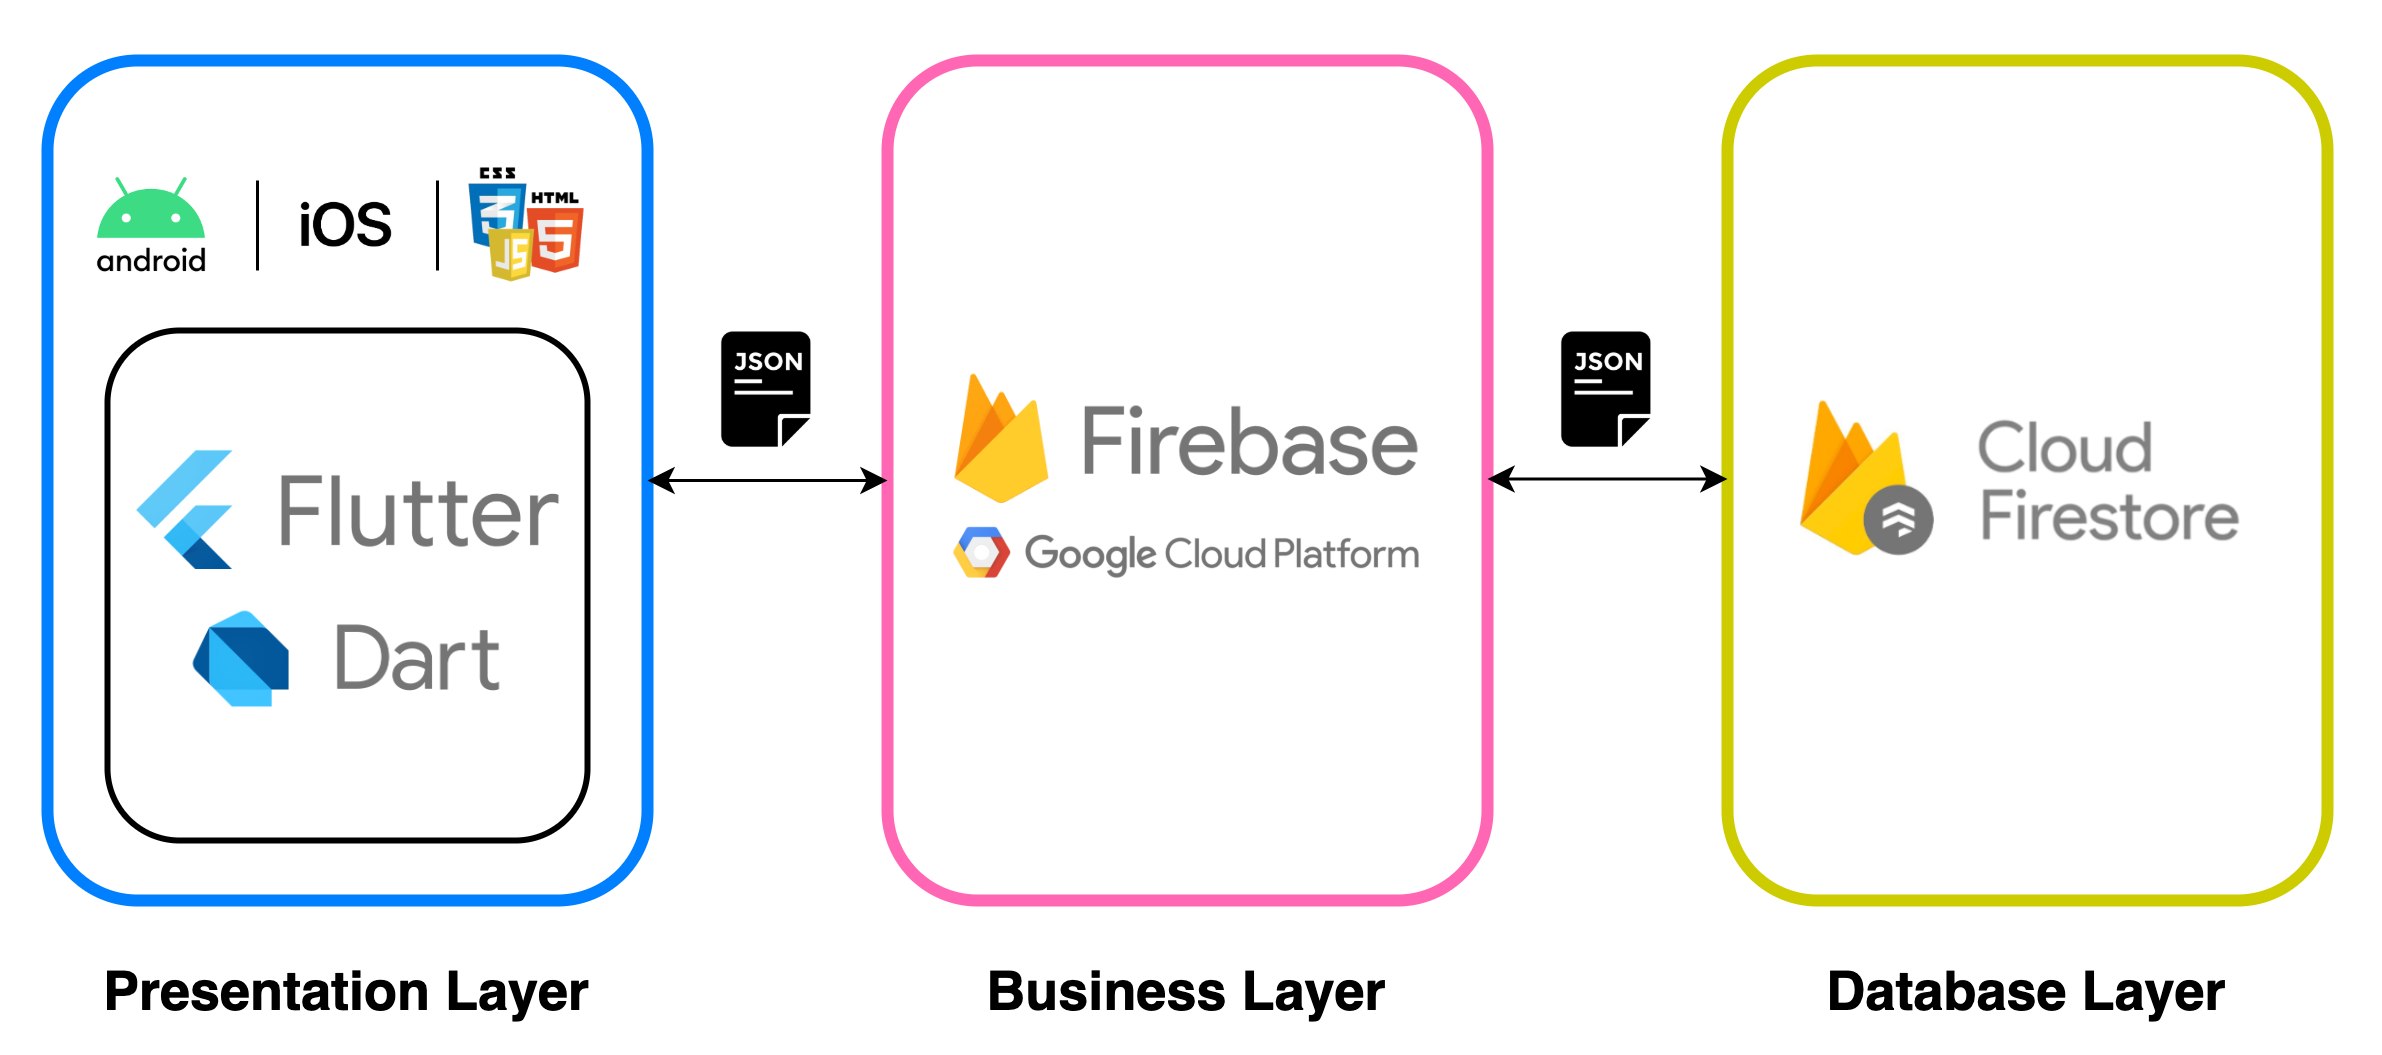
\includegraphics[width=0.8\textwidth]{./Images/arc.png}
\caption{Architecture of the Sterio system}
\label{fig:arc}
\end{figure}

\subsection{Database Layer}

The Database Layer is responsible for managing and storing all the data that it is used in the system. It receives information entered by the application's users and answers accordingly with the requested information from the Business Layer. ~\cite{Aarsten}

The first development step of the platform was the creation of an entity-relationship model so that we can model the database and determine which entities we need based on the medium-fidelity prototype described in section ~\ref{sec:userenactments}. The representation of this model, shown in Figure ~\ref{fig:eadiagram}, will help us visualize and conceptualize the system in the first stage, which will soothe the development difficulty and discard preliminary oversights.

\begin{figure}[h]
\centering
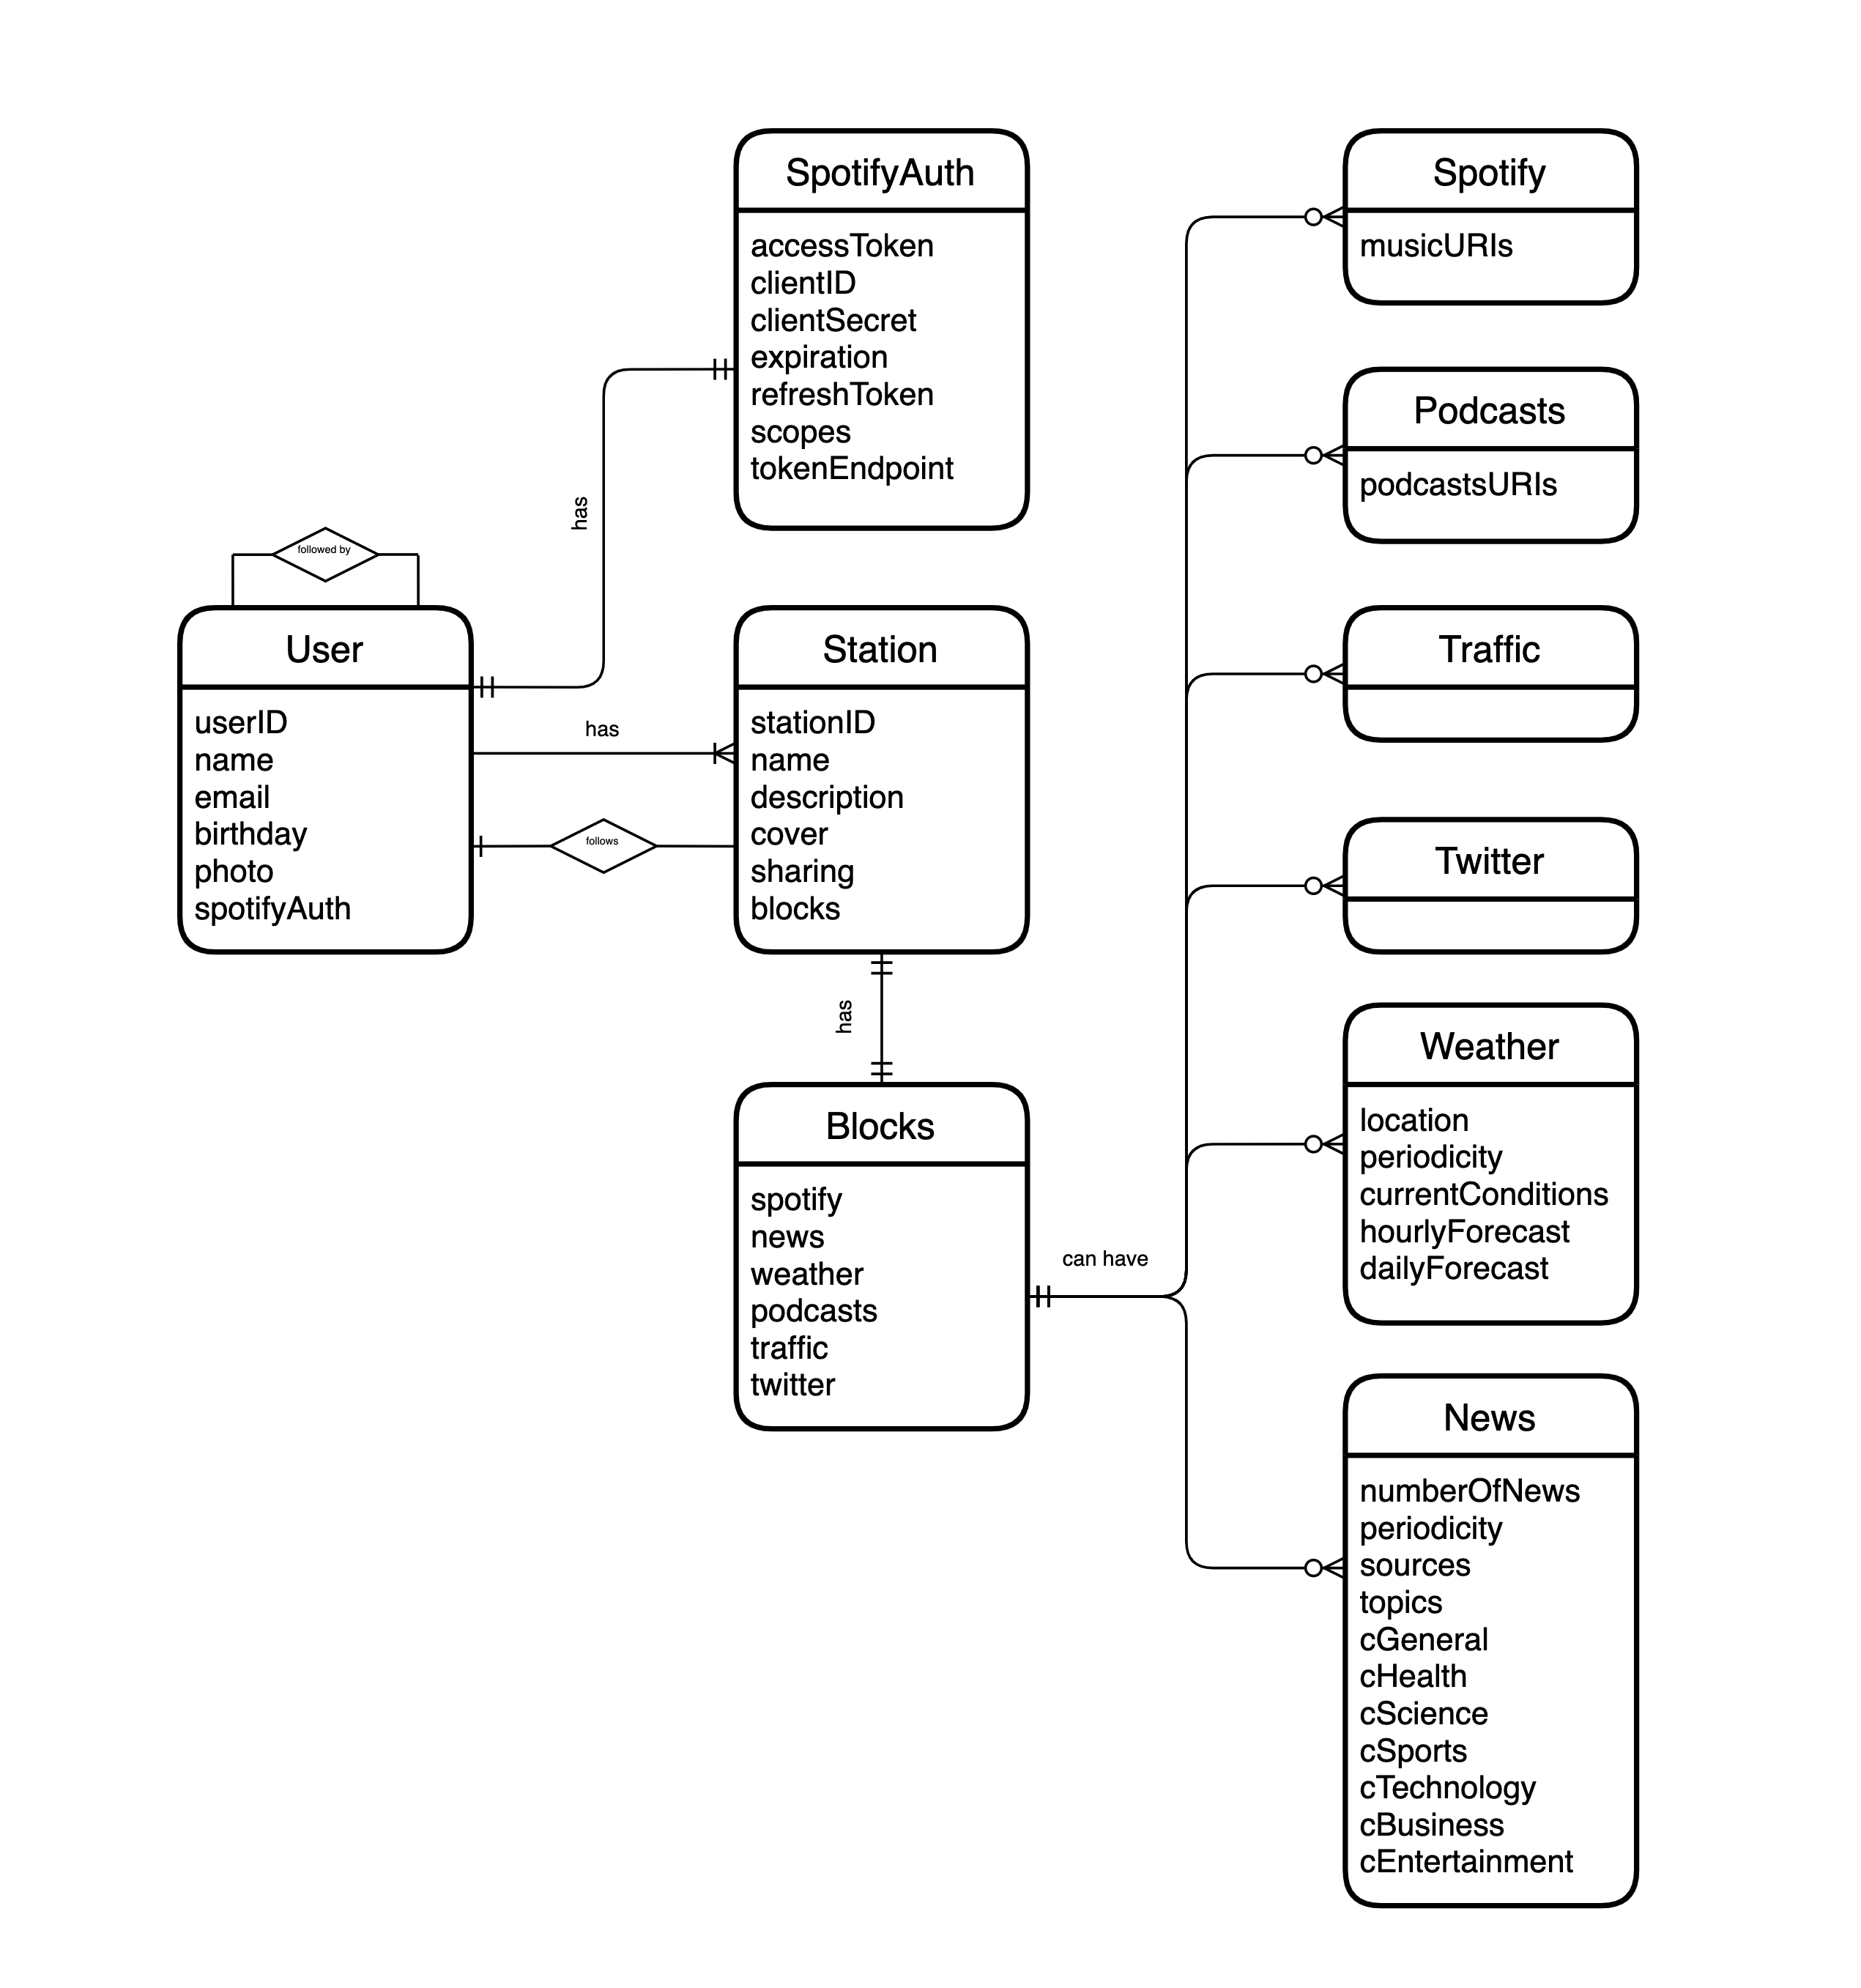
\includegraphics[width=0.8\textwidth]{./Images/ea.png}
\caption{Entity – Relationship Model of the Sterio system}
\label{fig:eadiagram}
\end{figure}


The implementation of the database was conducted using Google's Cloud Firestore~\footnote{Detailed information available on the platform's \href{https://firebase.google.com/products/firestore}{official website}.}, which is a NoSQL, document-oriented database. Being a NoSQL database, it provides several advantages, such as a non-relational and schema-less data model, low latency and high performance, highly scalable, and object-oriented programming that is easy and flexible to use. ~\cite{Stonebraker2010} Each document contains a set of key-value pairs, being optimized for storing sizable collections of small documents. It is a serverless document database that effortlessly scales to meet any demand, with no maintenance required, which accelerates the development of native cloud applications and lets developers focus their efforts on the most foreground layers of a system.

We chose to use Cloud Firestore due to its lean learning curve, ease-of-use, good performance, reliability, high scalability, and deep integration with other Google services that will also be used in the development of the platform. Furthermore, by using this technology, the system is prepared to be easily customized and to receive new data if the project has any changes in the way we approach some of its points.


\subsection{Business Layer}

The Business Layer is responsible to encode the real-world business rules that determine how data can be created, stored, and changed. It contrasts with the remainder of the software that might be concerned with lower-level details of managing a database or displaying the user interface, system infrastructure, or generally connecting various parts of the program. ~\cite{Aarsten}

For the Sterio platform, we chose to use Google's Firebase~\footnote{For more information on Google's Firebase and Cloud Platform services, visit its \href{https://firebase.google.com/}{official website}.} business logic features. Firebase is a \ac{MBaaS}, which is a model for providing web app and mobile app developers with a way to link their applications to backend cloud storage and \acp{API} exposed by back end applications while also providing features such as user management, push notifications, and integration with social networking services.

Firebase provides several pre-developed, robust, and reliable \acp{SDK} — such as authentication, hosting, storage, and app indexing — that helped us steer the focus of our development efforts to the design and conceiving of the user experience and interface. As with Cloud Firestore, it integrates thoroughly with other Google services, while also allowing the configuration of third-party \acp{API} that will be used in the context of our project.


\subsection{Presentation Layer}

The third and final layer of the system is the Presentation Layer, which is responsible for the interaction between the user and the system. ~\cite{Aarsten} This layer will interact with the business layer through calls to the Firebase service.

Based on the preliminary user research presented in Section ~\ref{chap:userresearch}, and corroborating with the data shown in Figure ~\ref{chart:devices}, most users listen to music streaming services on their smartphone. Furthermore, as we want our platform to be easily accessible on the go, we focused our efforts in analyzing the most popular mobile development frameworks to develop our platform on.

\begin{figure}
	\centering
	\caption{Share of internet users who have used a music streaming services in the last month worldwide in 2nd quarter 2017, by device (Statista / GlobalWebIndex)}
	\label{chart:devices}
	\begin{bchart}[step=10,max=45,unit=\%,width=0.8\textwidth]
        \bcbar[text=Smartphone (Mobile)]{39}
            \smallskip
        \bcbar[text=PC / Laptop]{30}
            \smallskip
        \bcbar[text=Tablet]{8}
    \end{bchart}
\end{figure}


We chose to develop the Sterio platform using Flutter~\footnote{To learn more about the Flutter framework, consult the \href{https://flutter.dev/}{official website}.}, which is an \ac{UI} toolkit for building natively compiled applications for mobile, web, and desktop from a single codebase. Flutter apps are written in the Dart~\footnote{For more information on the Dart programming language, visit its \href{https://dart.dev/}{official website}.} programming language and make use of many of the language's more advanced features. ~\cite{Payne2019}

In the context of our project, Flutter has some key advantages over other technologies. To start, although it has been built as a mobile-first toolkit in the first stage, Flutter is now a cross-platform development tool that allows the development of mobile (on the Android and iOS operating systems) and desktop apps without compounding changes to the codebase. This ensures that our platform renders well on a variety of devices and windows or screen sizes, without limiting our endeavors. ~\cite{H.GillbertMiller2011} Secondly, in comparison with other mobile frameworks, Flutter reduces the code development time by a wide margin. In a large and complex project such as ours, this is a crucial advantage that will lead us to a robust final product without the need for allocating umpteen resources. Finally, Flutter offers a variety of advanced tools that allow us to achieve a great user experience and interface design, which will help us achieve our goals. ~\cite{Payne2019}

% #############################################################################

\section{Functional Prototype}

Based on the medium-fidelity prototype presented in Section ~\ref{sec:userenactments}, the last — and most important — step of the development cycle was to construct a functional prototype with a fully-working set of features. This prototype should resemble as close as possible to the final representation of the system. 

In the following subsections, we describe in detail all functionalities, components, screens, implementations, and technical facets of the Sterio system, as well as the design implications and limitations faced during the development of the prototype.

\subsection{Login, Signup, and Authentication}

The first interaction the user has with the Sterio platform is the login / signup screen, shown in Figure ~\ref{fig:login1}. There, the user can choose to login with an Apple or Facebook account, or with an e-mail. If the user chooses to use one of the first two methods, an in-app browser window is shown so that the user can enter the required credentials. If the user chooses to use an e-mail as a sign up method, the screen shown in ~\ref{fig:login2} is presented.

\begin{figure}[htbp]
	\centering
	\subfigure[Login / Signup screen]{\label{fig:login1}
	\frame{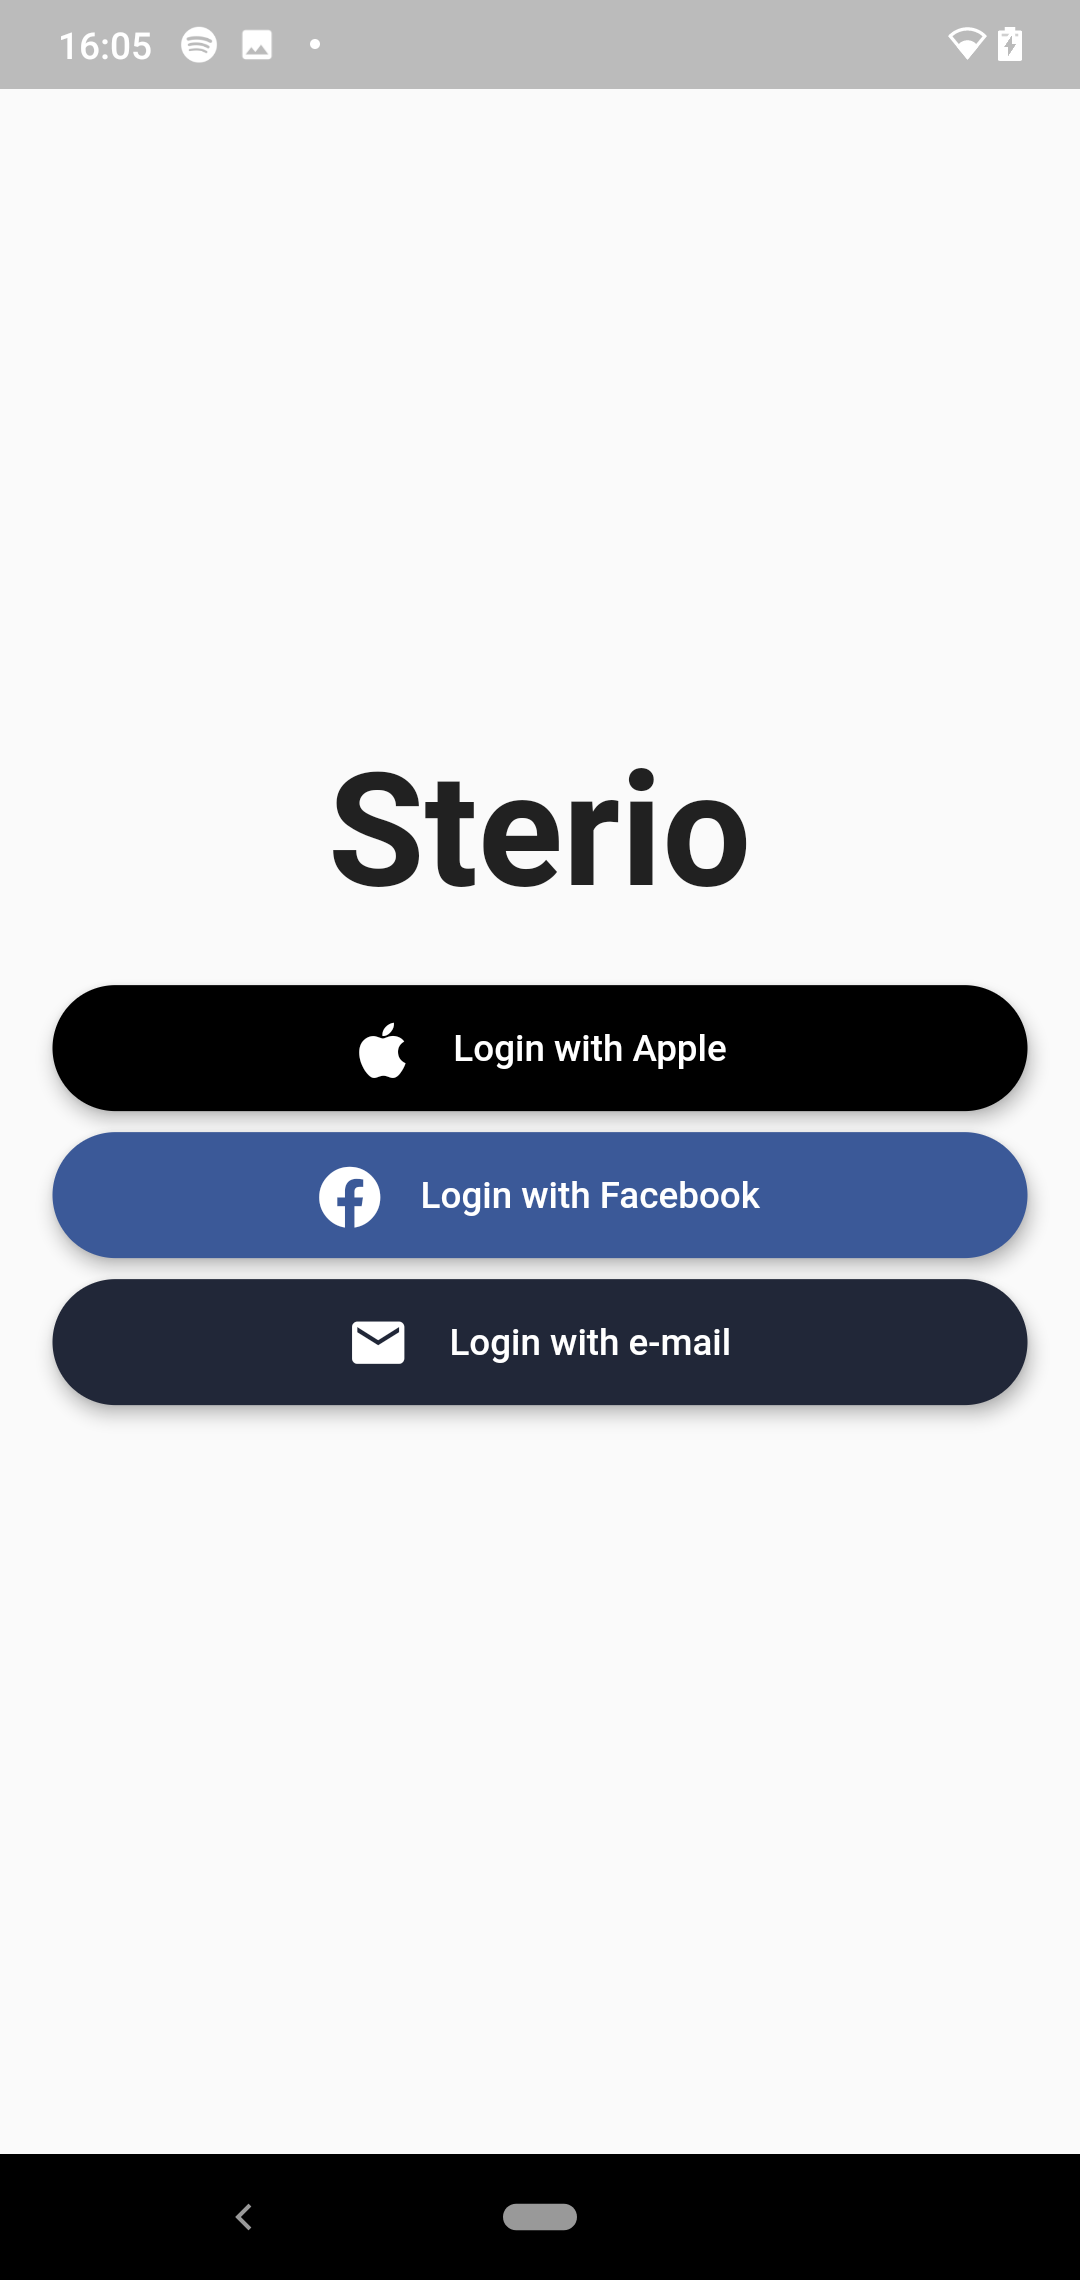
\includegraphics[width=0.29\textwidth]{./Images/screenshots/login1.png}}} \qquad
	\subfigure[Login with e-mail]{\label{fig:login2}
	\frame{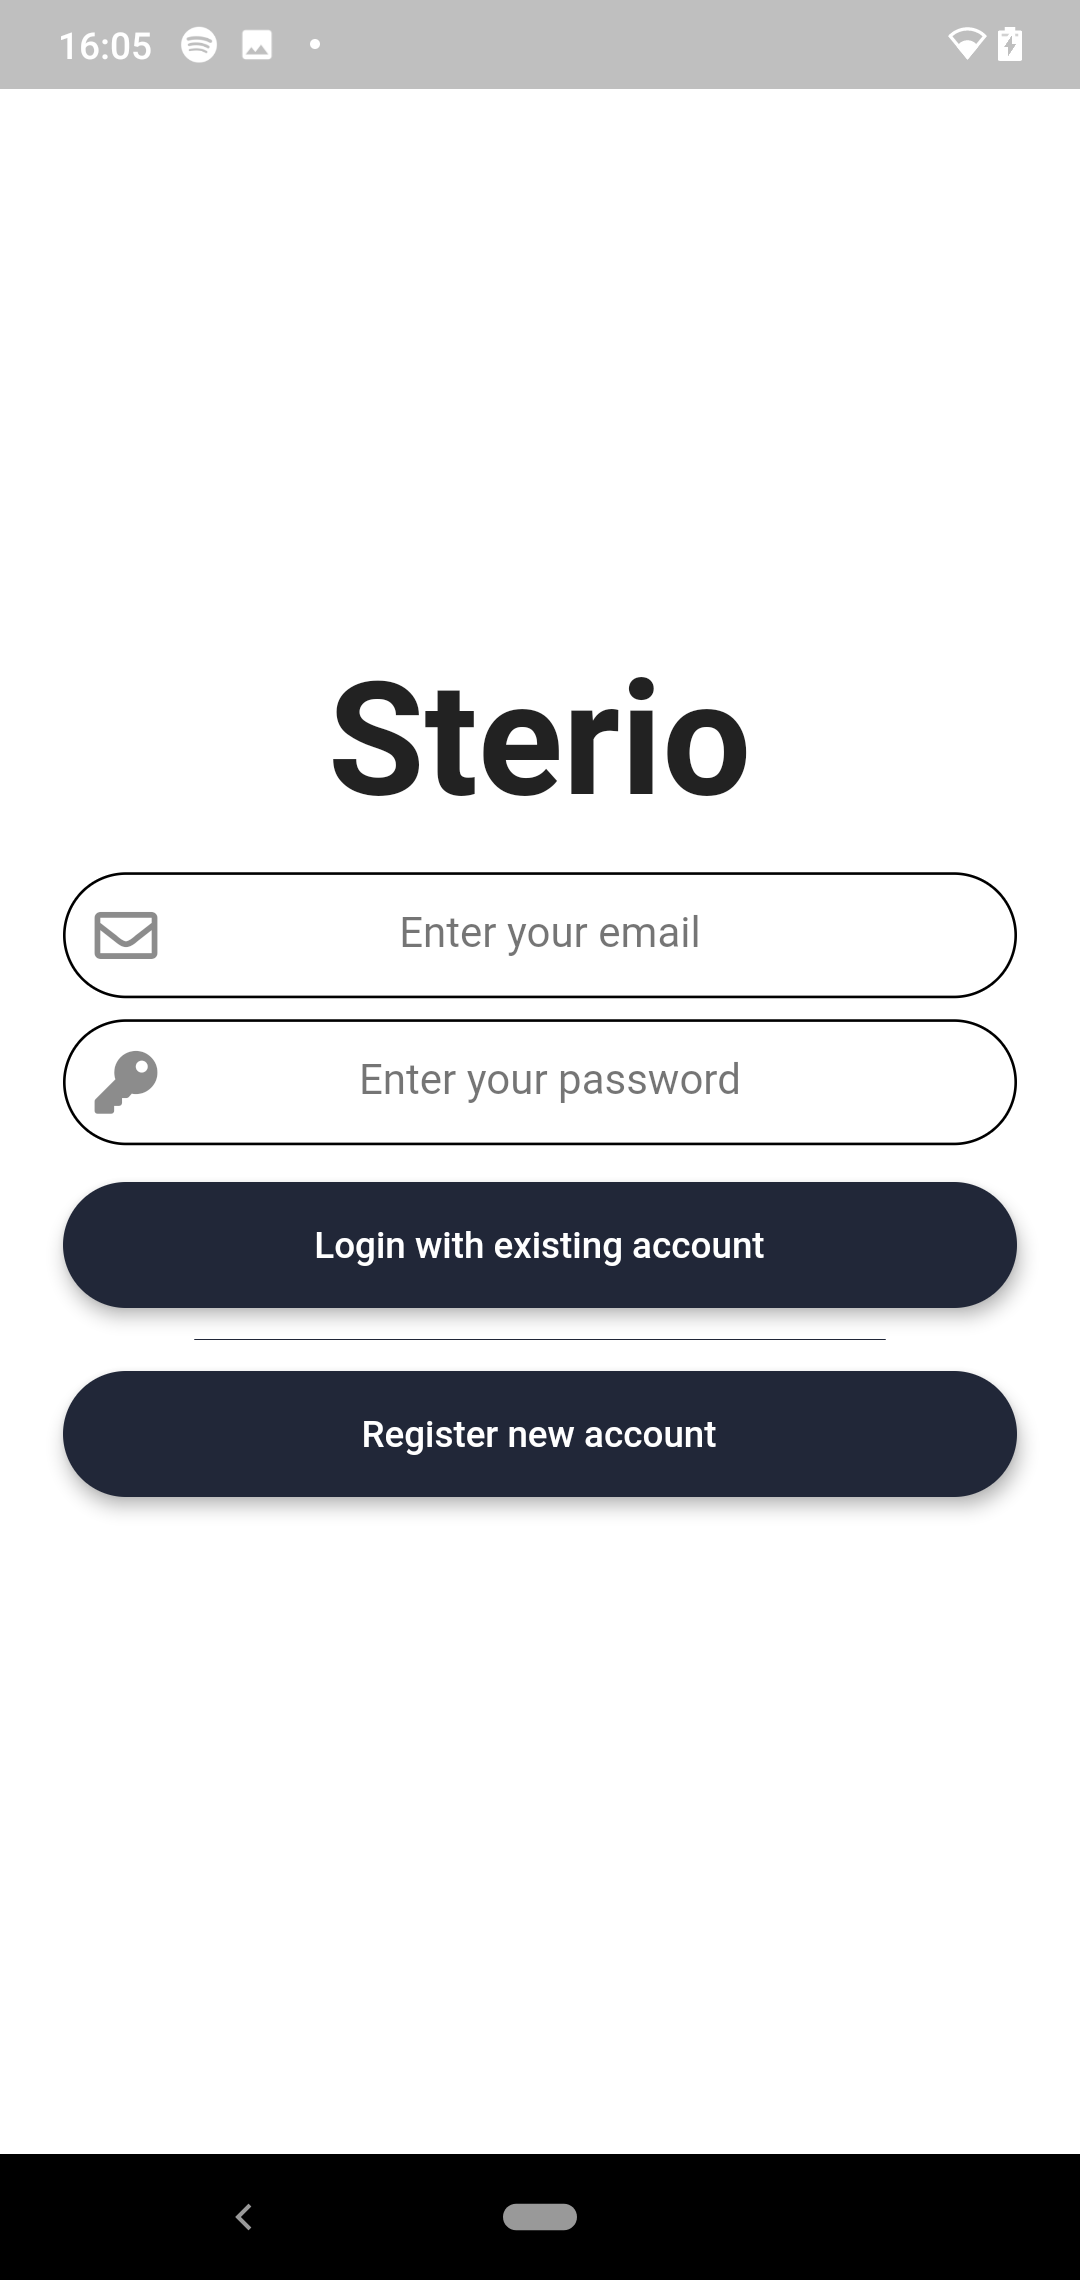
\includegraphics[width=0.29\textwidth]{./Images/screenshots/login2.png}}} \qquad
	\subfigure[Spotify authentication]{\label{fig:auth}
	\frame{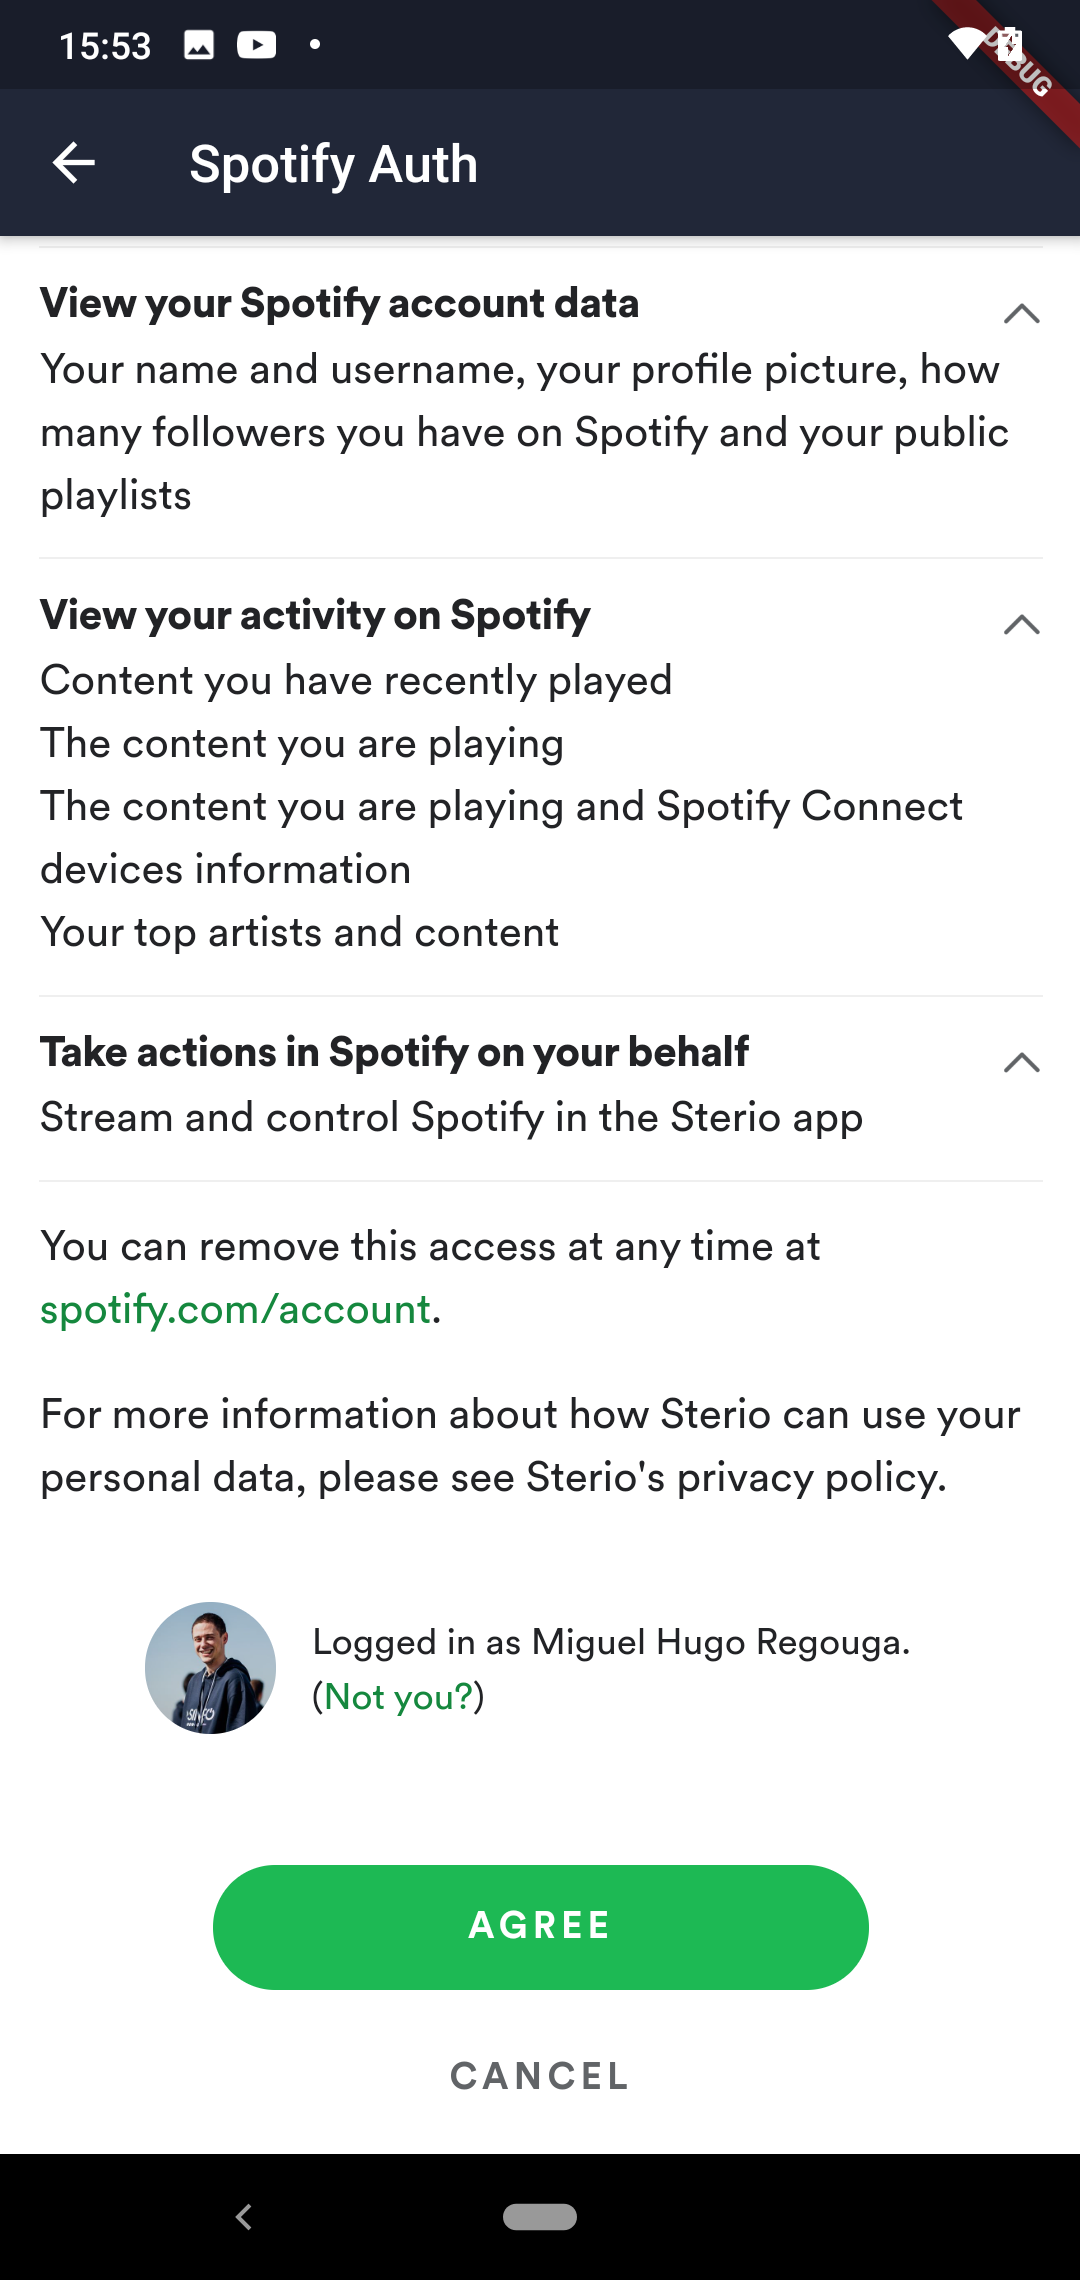
\includegraphics[width=0.29\textwidth]{./Images/screenshots/auth.png}}} \qquad
	\caption{Login, Signup, and Spotify authentication screens}
	\label{fig:lss}
\end{figure}

As the system integrates with a Spotify Premium account, it is also necessary that the user authenticates with the music streaming service, so that we can take advantage of its ~\ac{API}. To do so, an in-app browser window, shown in Figure ~\ref{fig:auth}, is also presented to the user. This is a one-time step, as the system stores the necessary ~\ac{API} parameters in the database and automatically logs in the user in future usages.

\subsection{'Home' and 'Search' Screens}

After logging in, the user is prompted with the 'Home' screen, shown in Figure ~\ref{fig:homes}, which is the first and most foregrounding screen of the platform. In this screen, the user can quickly play a station based on a recent activity, friends activity, top charts, or other relevant information tailored to the user's taste and usability history. In this screen, the user can also change the settings and preferences of the app, as well as of the signed-in account. Finally, the user can also enter the "Car Mode" of the system, which transforms the ~\ac{UI} in a stripped-down, non-distracting, and easy way for the user to control playback while driving.

\begin{figure}[htbp]
	\centering
	\subfigure['Home' screen]{\label{fig:homes}
	\frame{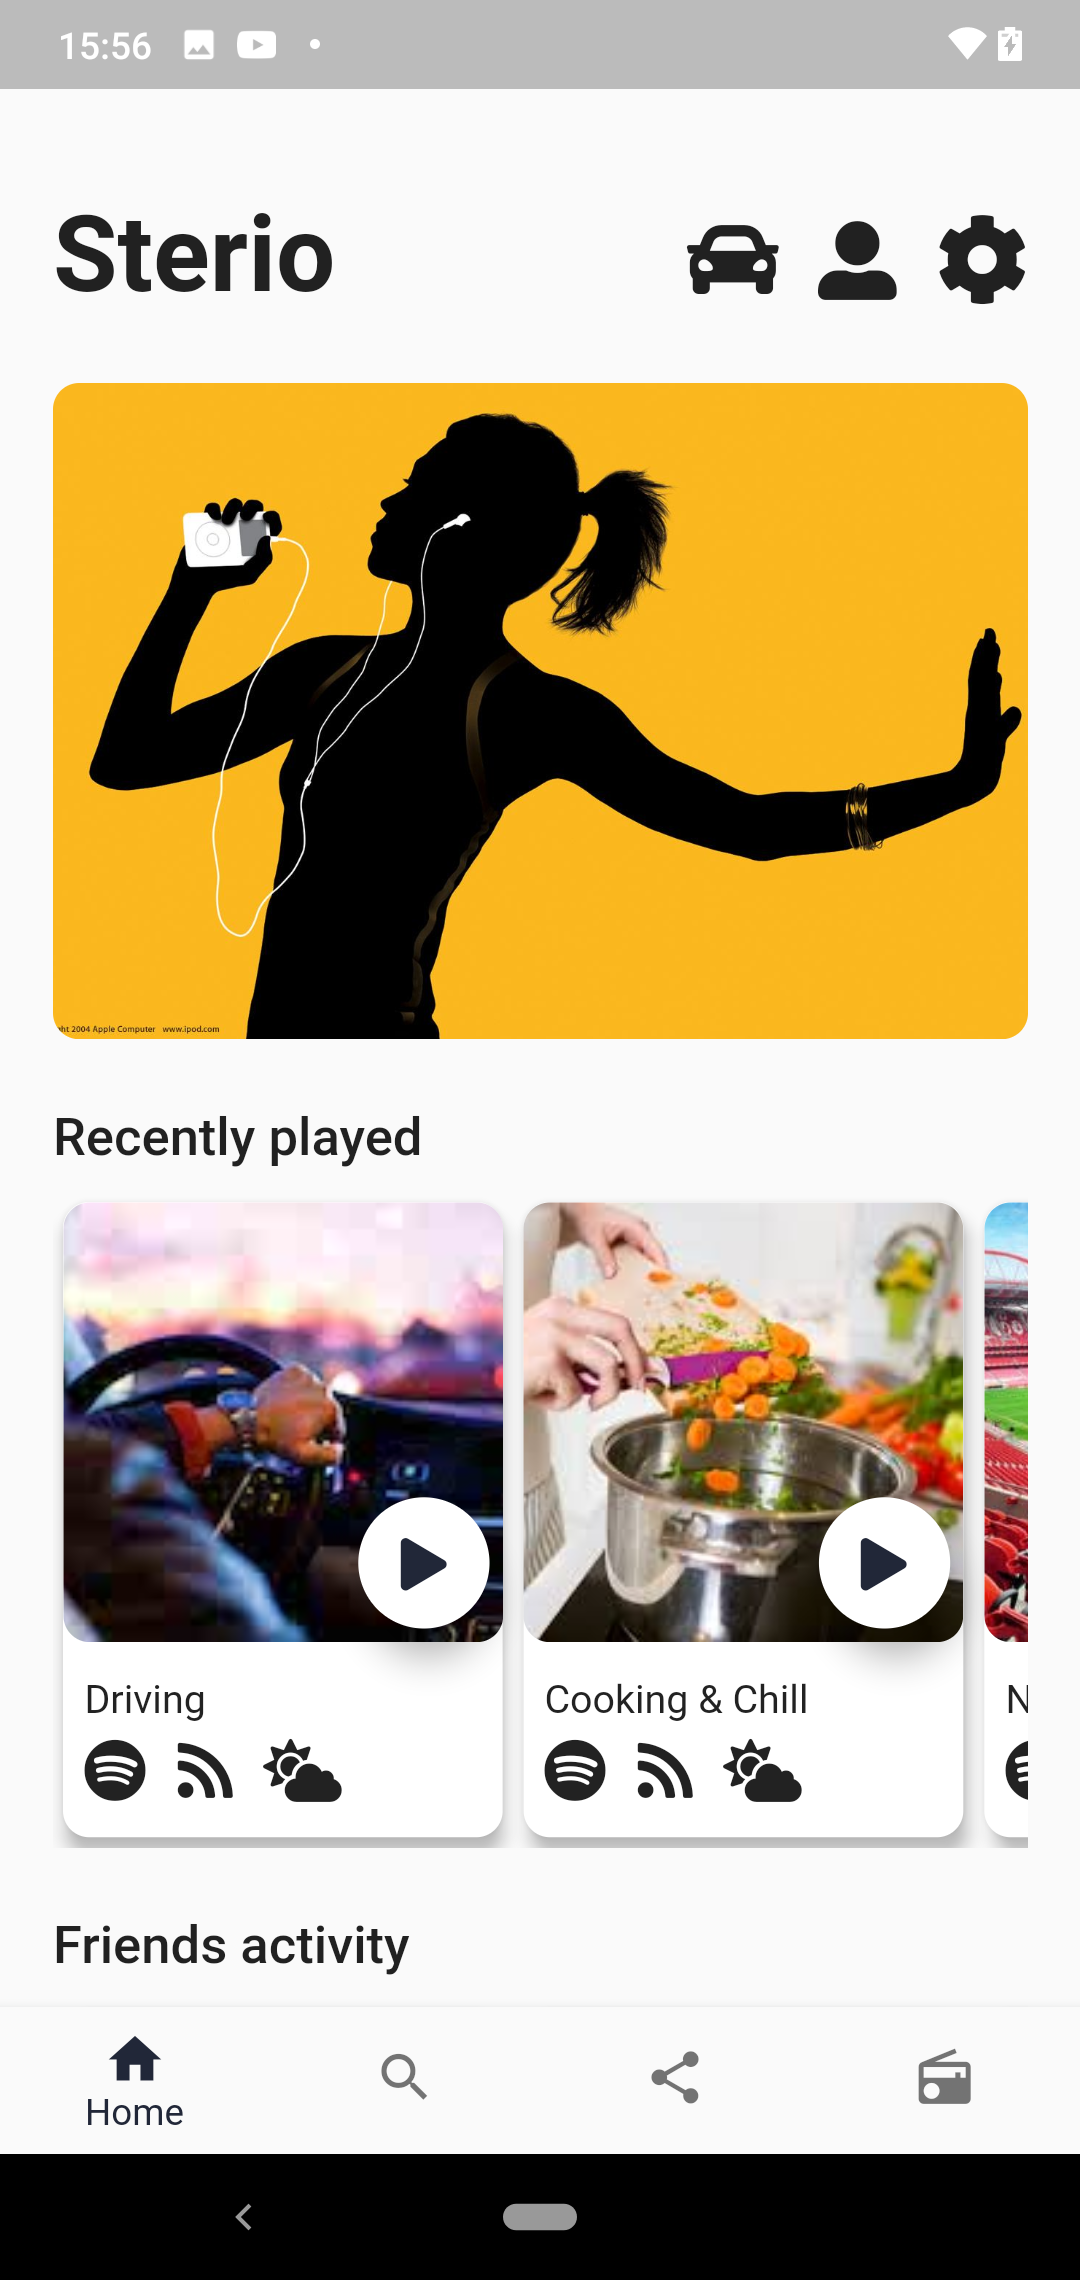
\includegraphics[width=0.29\textwidth]{./Images/screenshots/home.png}}} \qquad
	\subfigure['Search' screen]{\label{fig:searchs1}
	\frame{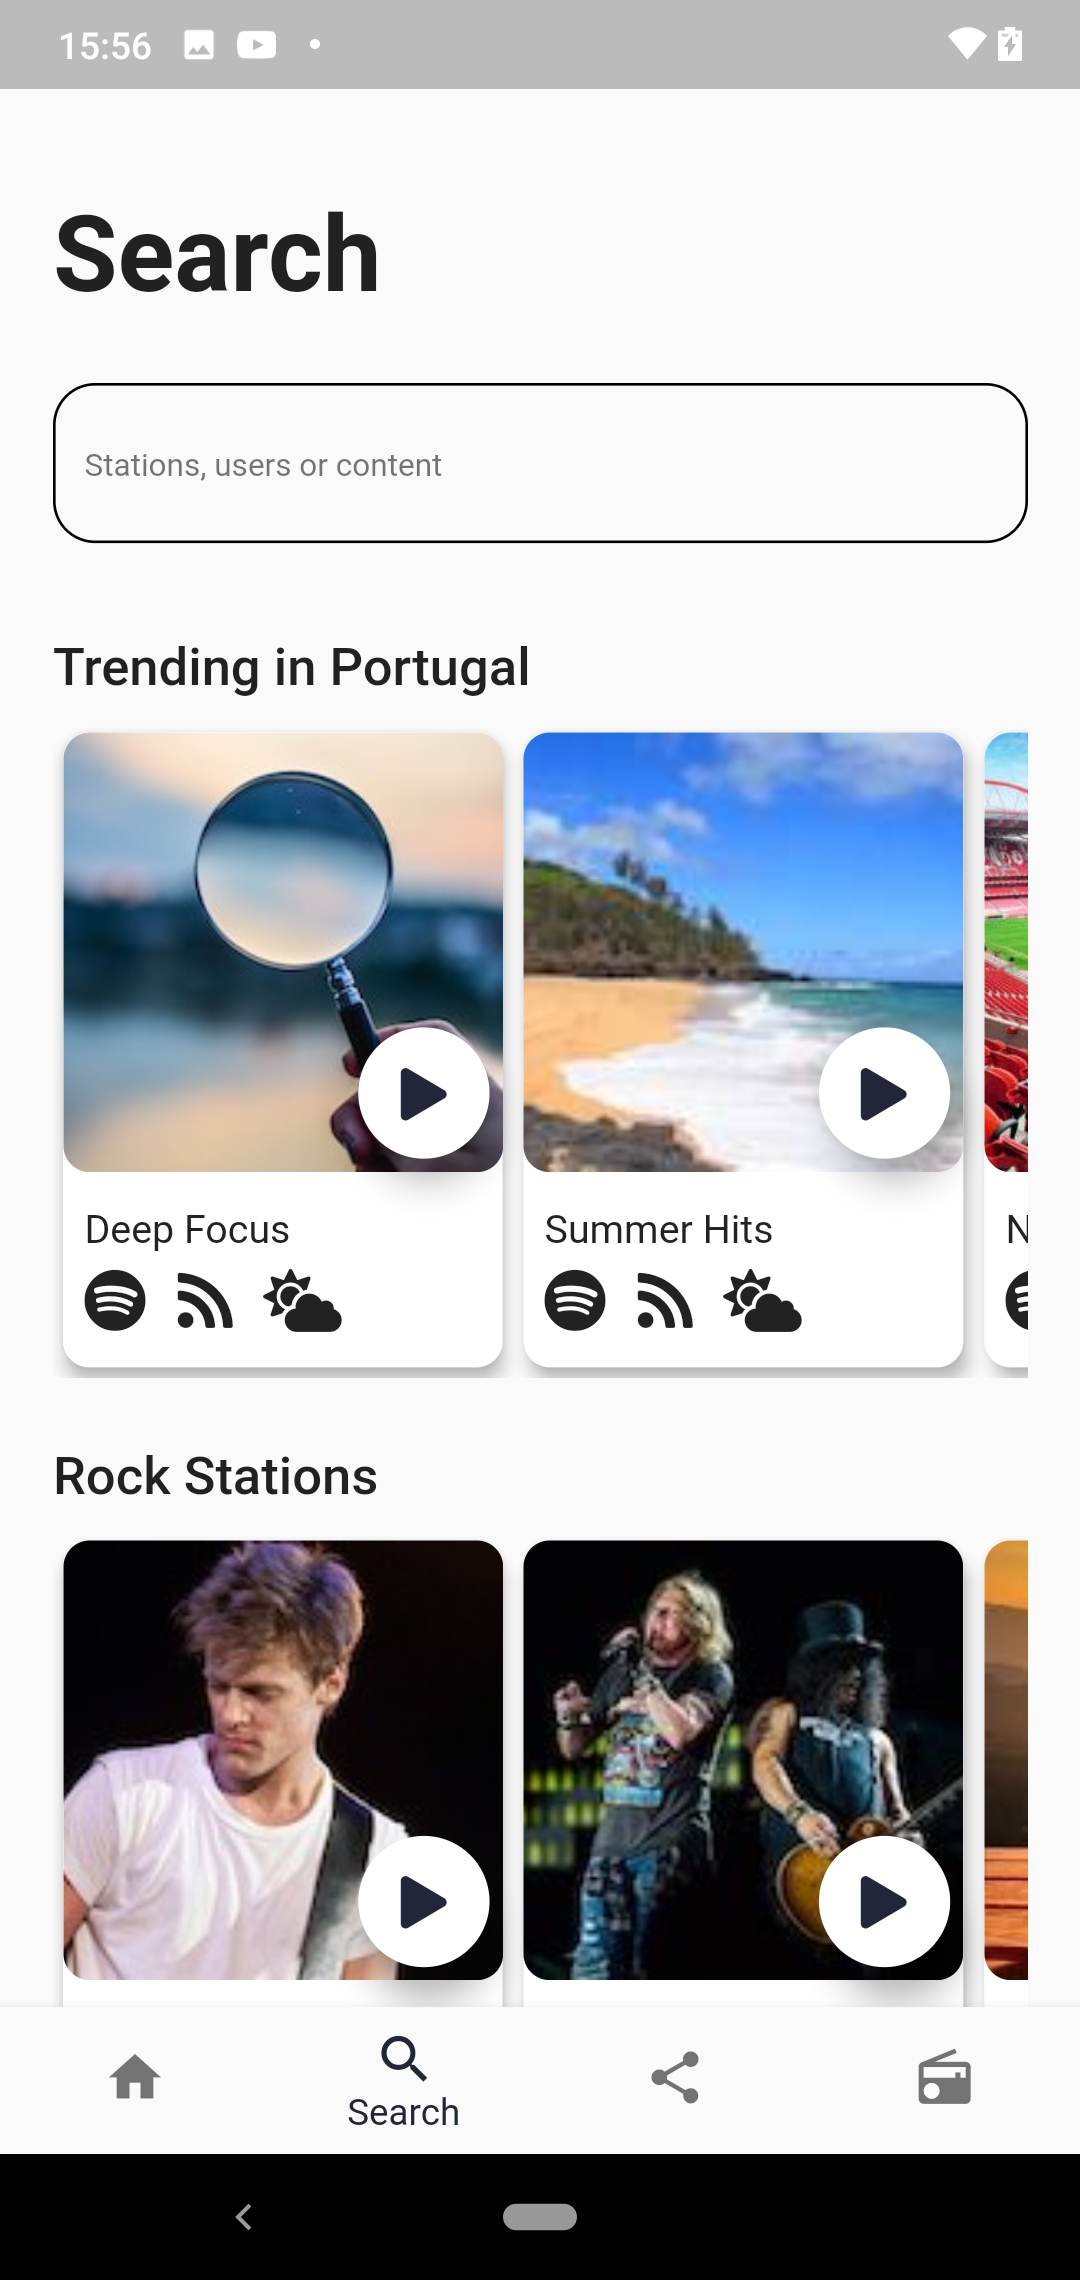
\includegraphics[width=0.29\textwidth]{./Images/screenshots/search.png}}} \qquad
	\caption{'Home' and 'Search' screens}
	\label{fig:mfp1}
\end{figure}

In the 'Search' screen, shown in Figure ~\ref{fig:searchs1}, the user can search for a specific station, content, or even other users to follow and check their profiles. In the same screen some suggestions are also shown, based on the most searched items and trending stations a given location.


\subsection{'Social' Screen}

\begin{figure}[htbp]
	\centering
	\subfigure[Social screen showing friends that are playing a station]{\label{fig:social1}
	\frame{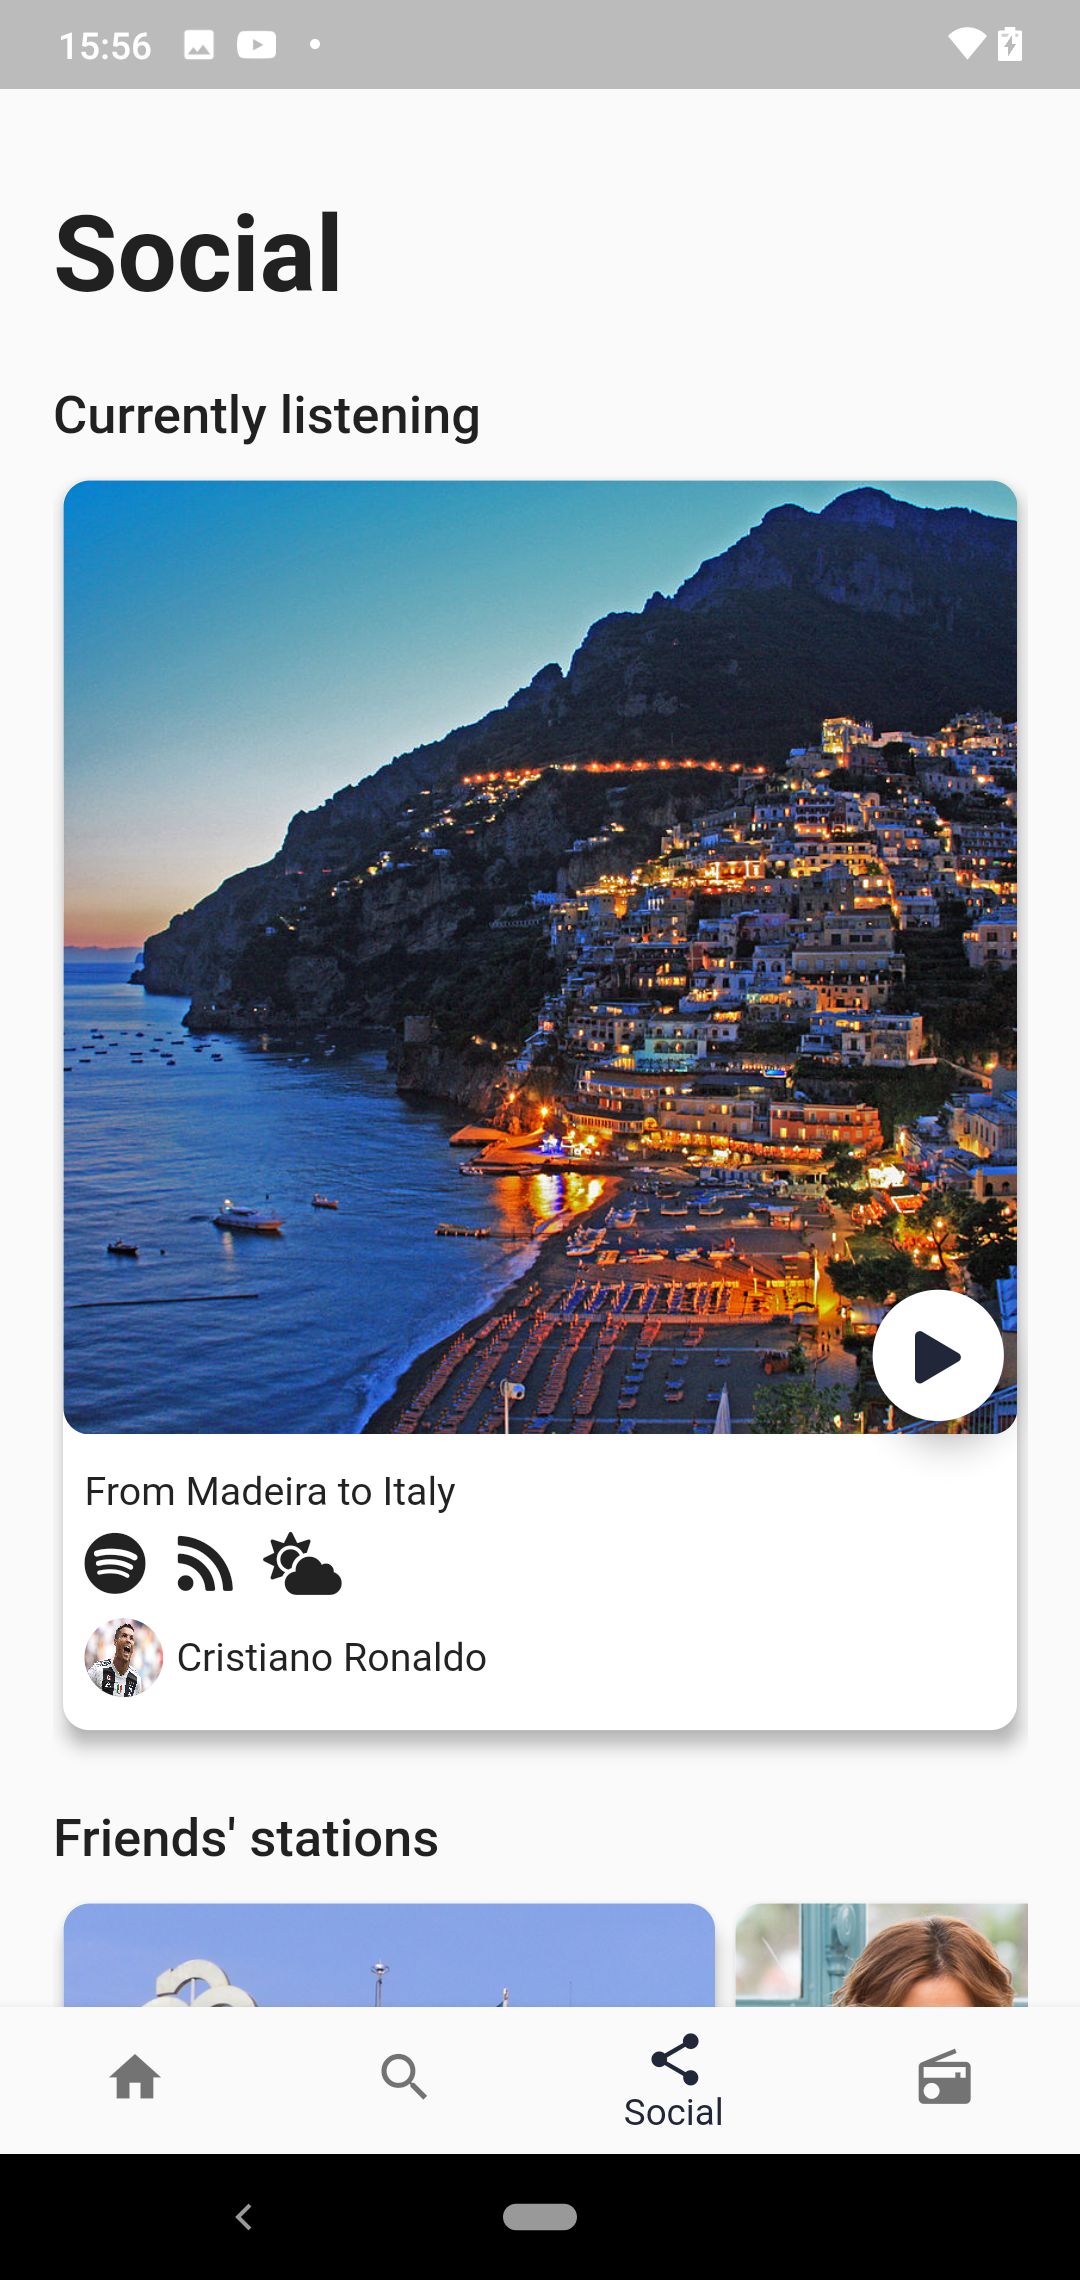
\includegraphics[width=0.29\textwidth]{./Images/screenshots/social1.png}}} \qquad
	\subfigure[Social screen with following suggestions]{\label{fig:social2}
	\frame{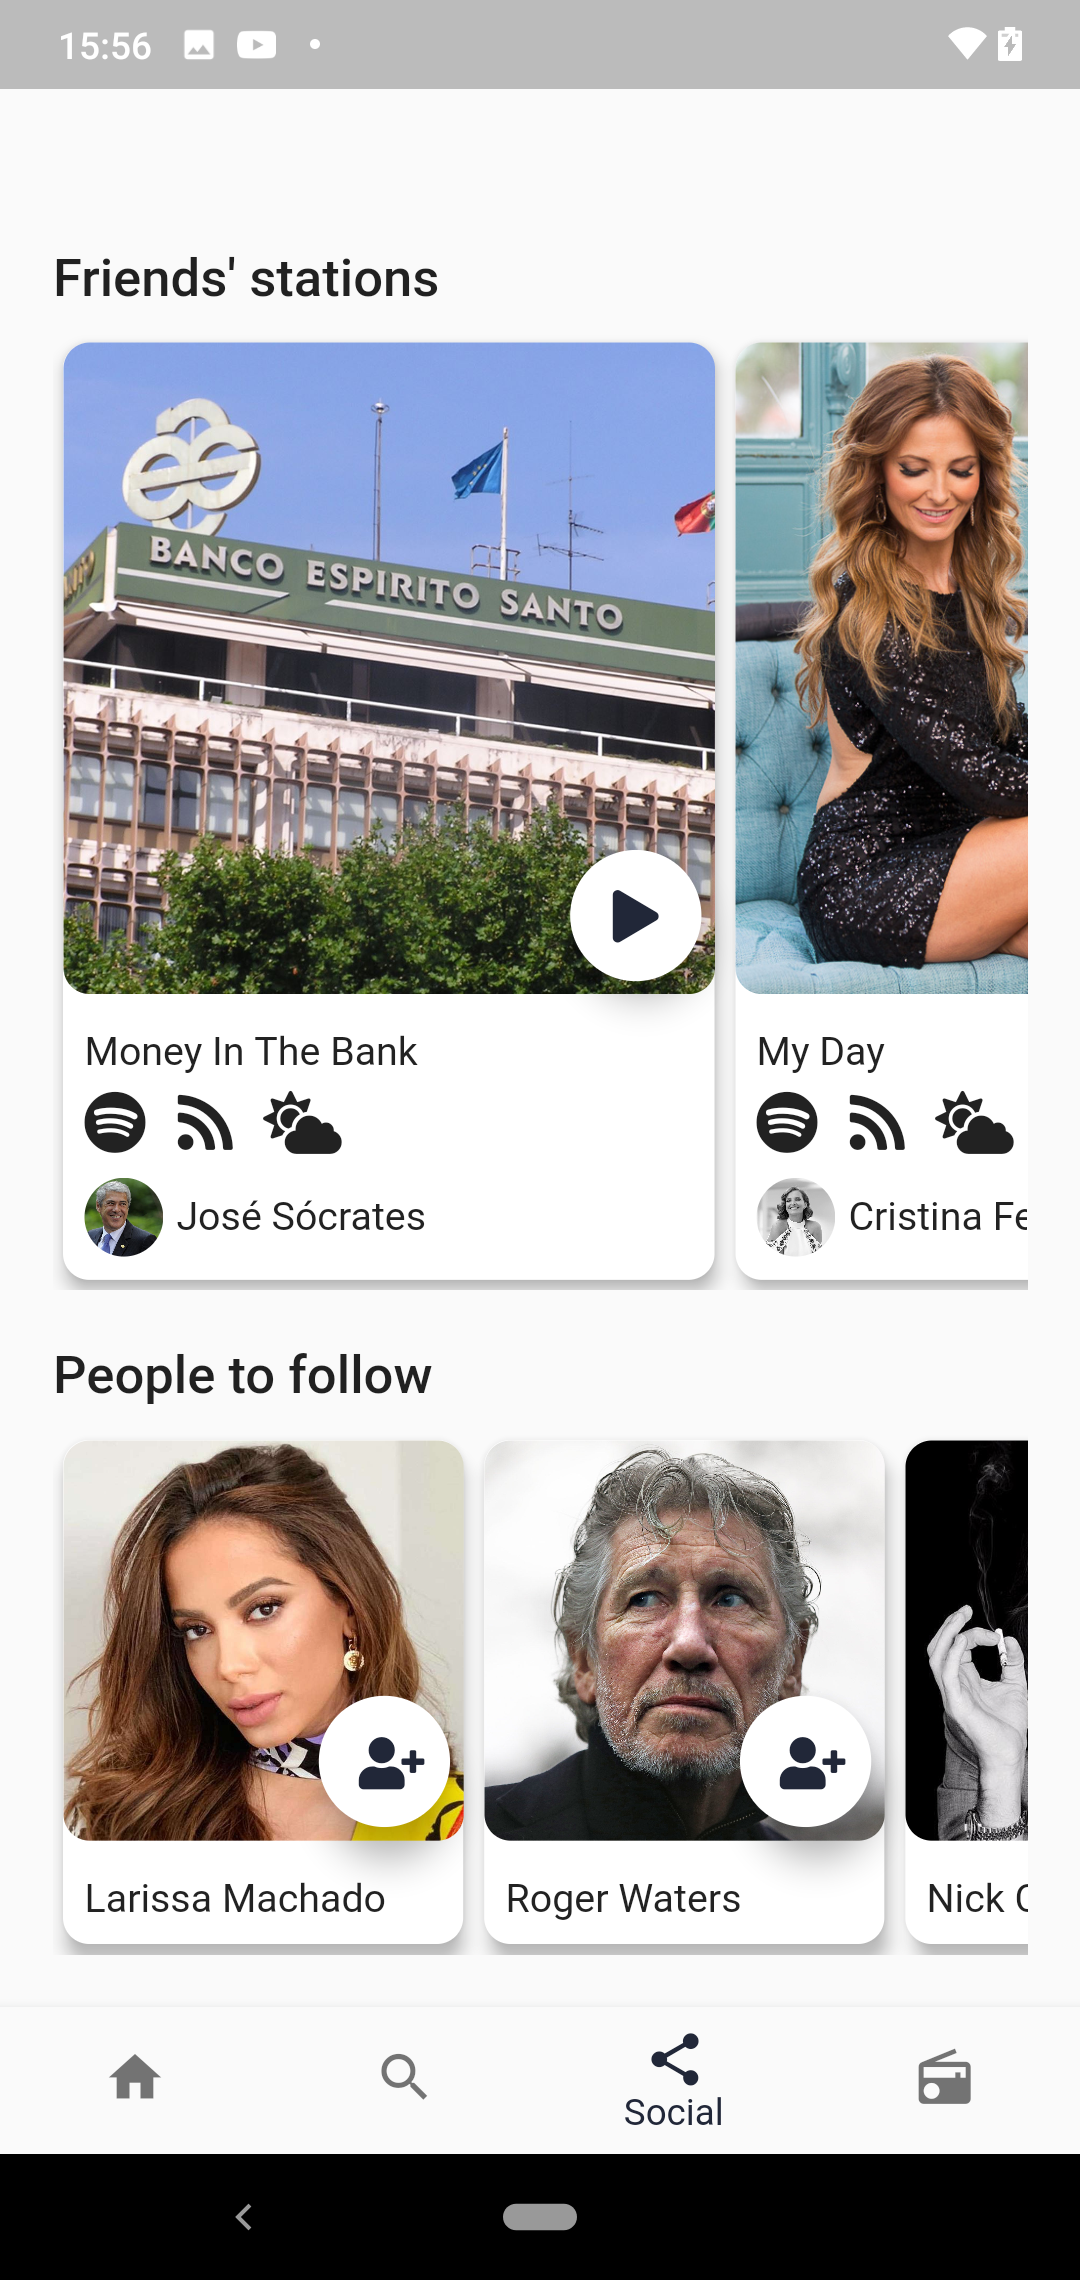
\includegraphics[width=0.29\textwidth]{./Images/screenshots/social2.png}}} \qquad
	\caption{'Social' screen}
	\label{fig:mfp1}
\end{figure}

\subsection{'My Stations' Screen}

\begin{figure}[h]
\centering
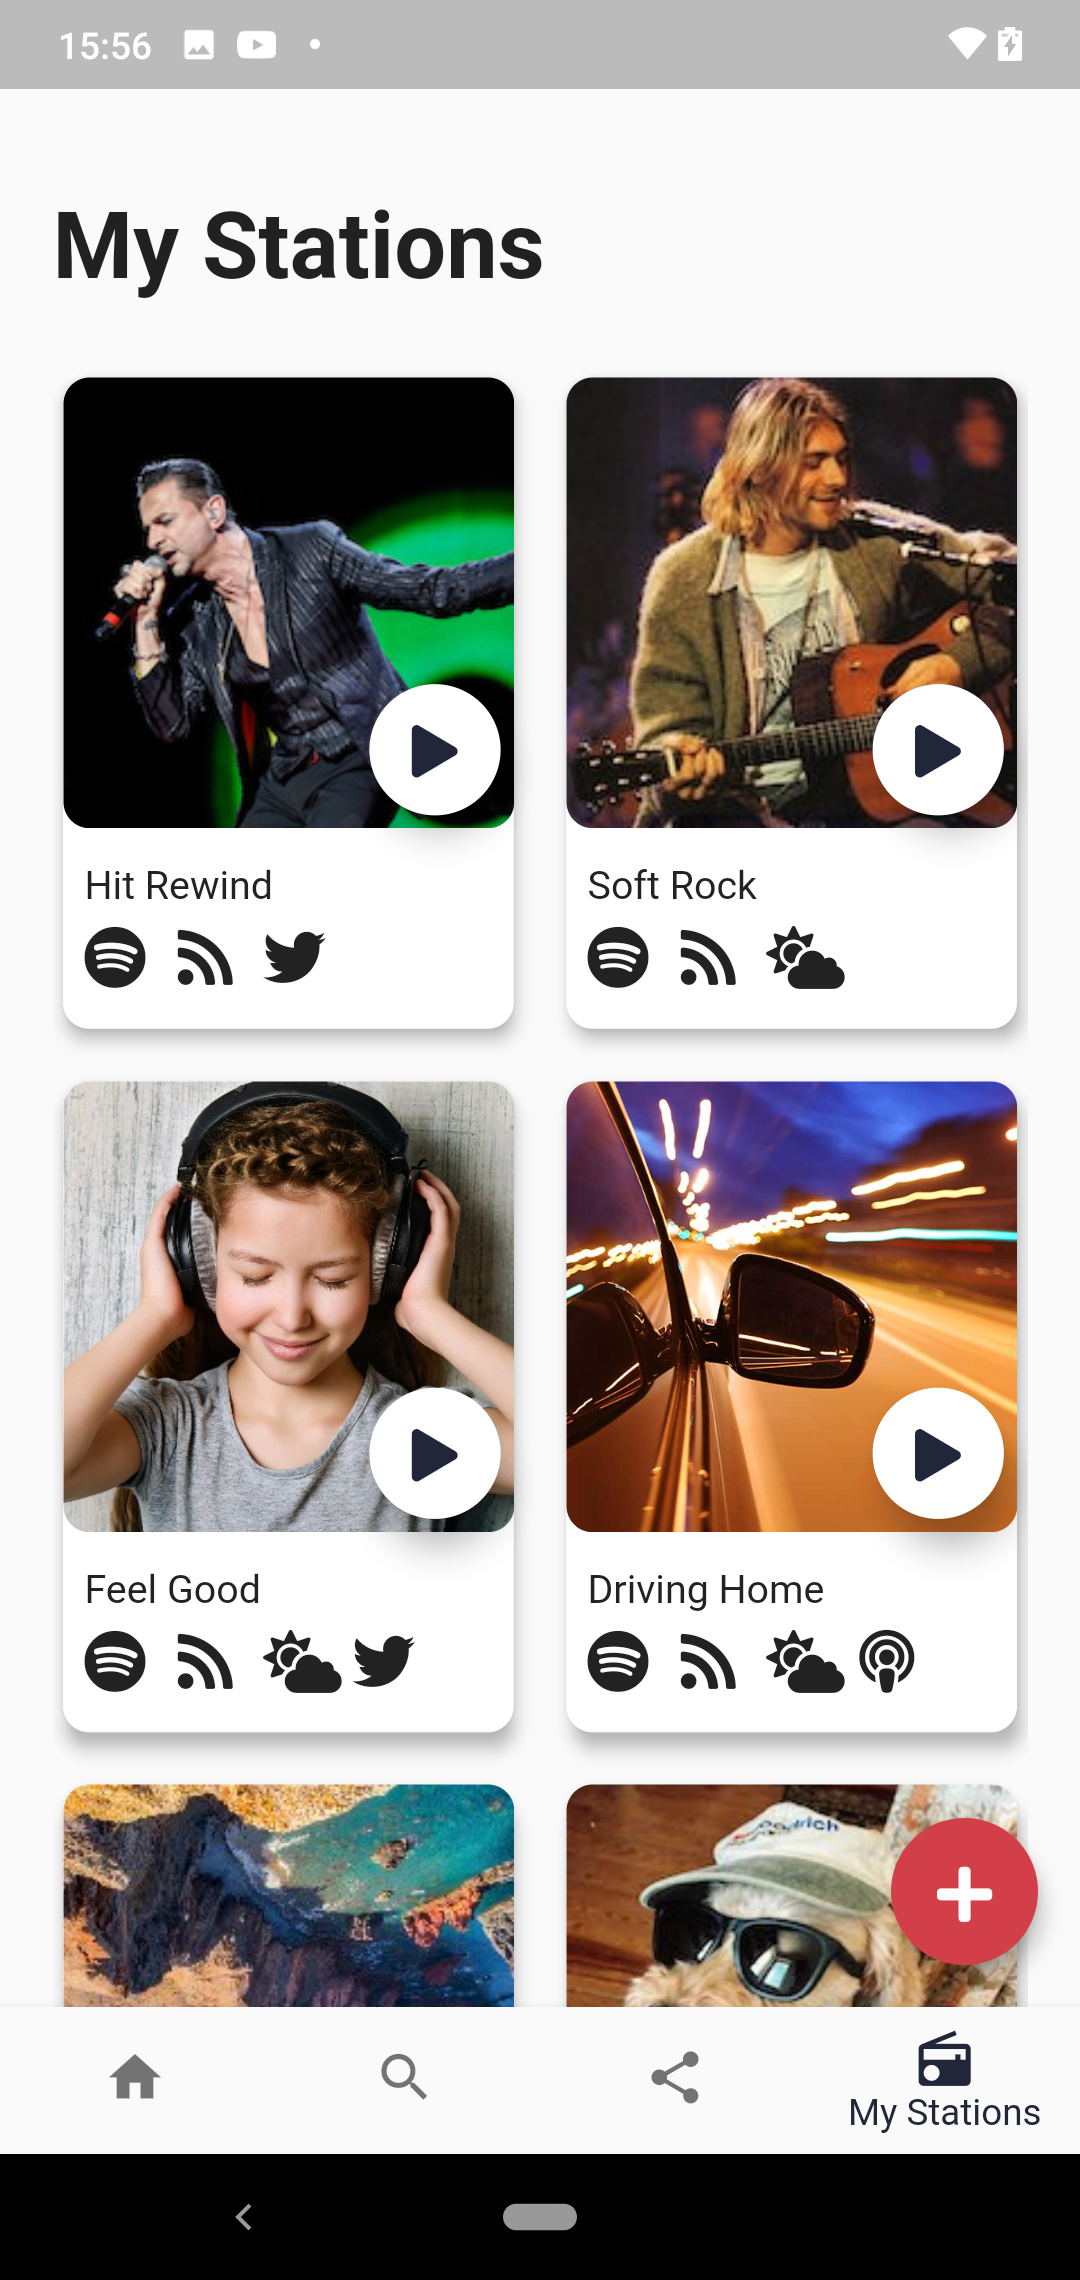
\includegraphics[width=0.29\textwidth]{./Images/screenshots/mys.png}
\caption{'My Stations' screen}
\label{fig:mys}
\end{figure}


\subsection{Creating a New Station}

\begin{figure}[htbp]
	\centering
	\subfigure[Step 1 (stations' details)]{\label{fig:ns1}
	\frame{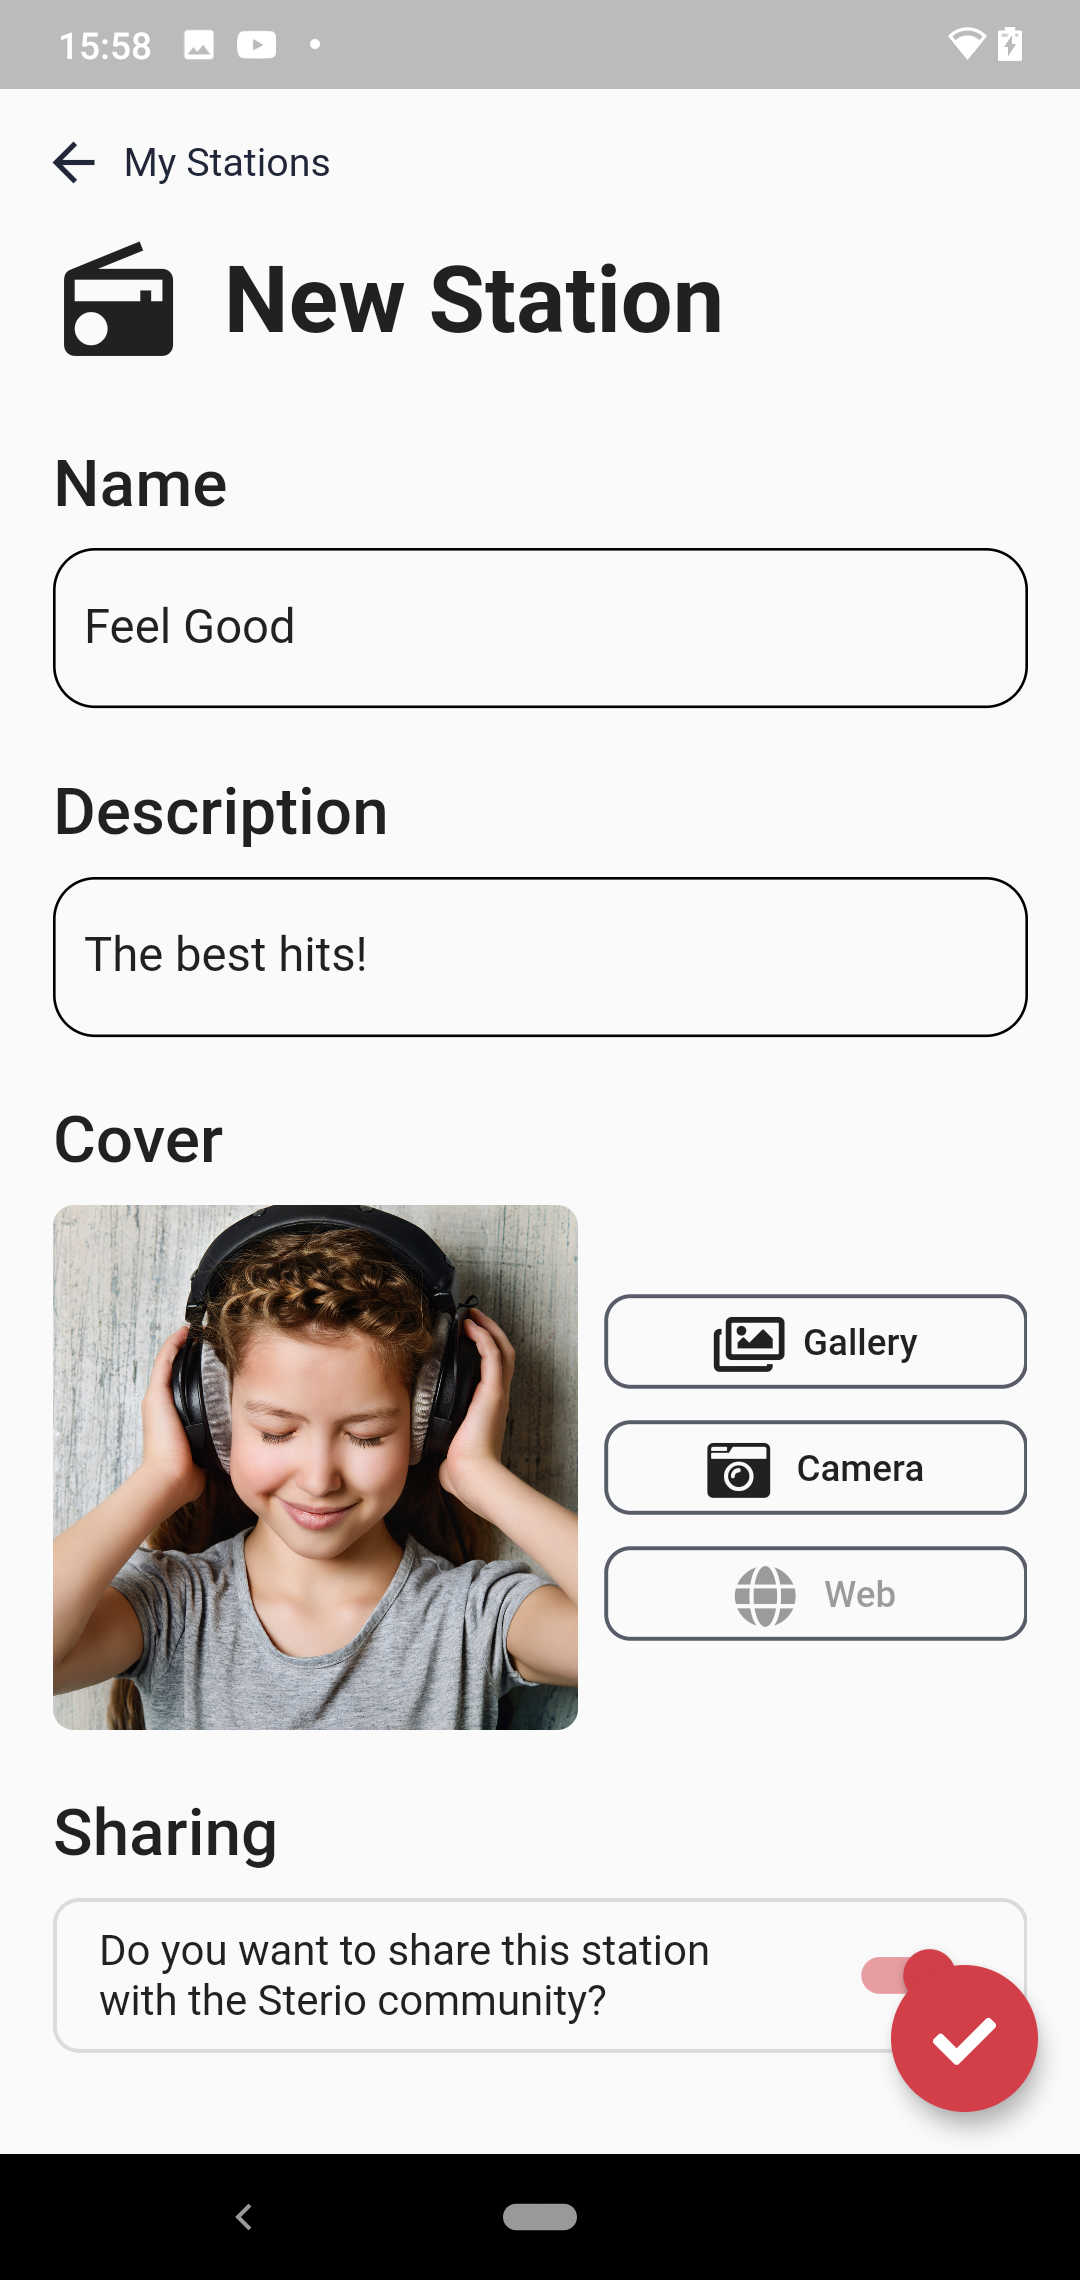
\includegraphics[width=0.29\textwidth]{./Images/screenshots/newstation1.png}}} \qquad
	\subfigure[Step 2 (adding blocks)]{\label{fig:ns2}
	\frame{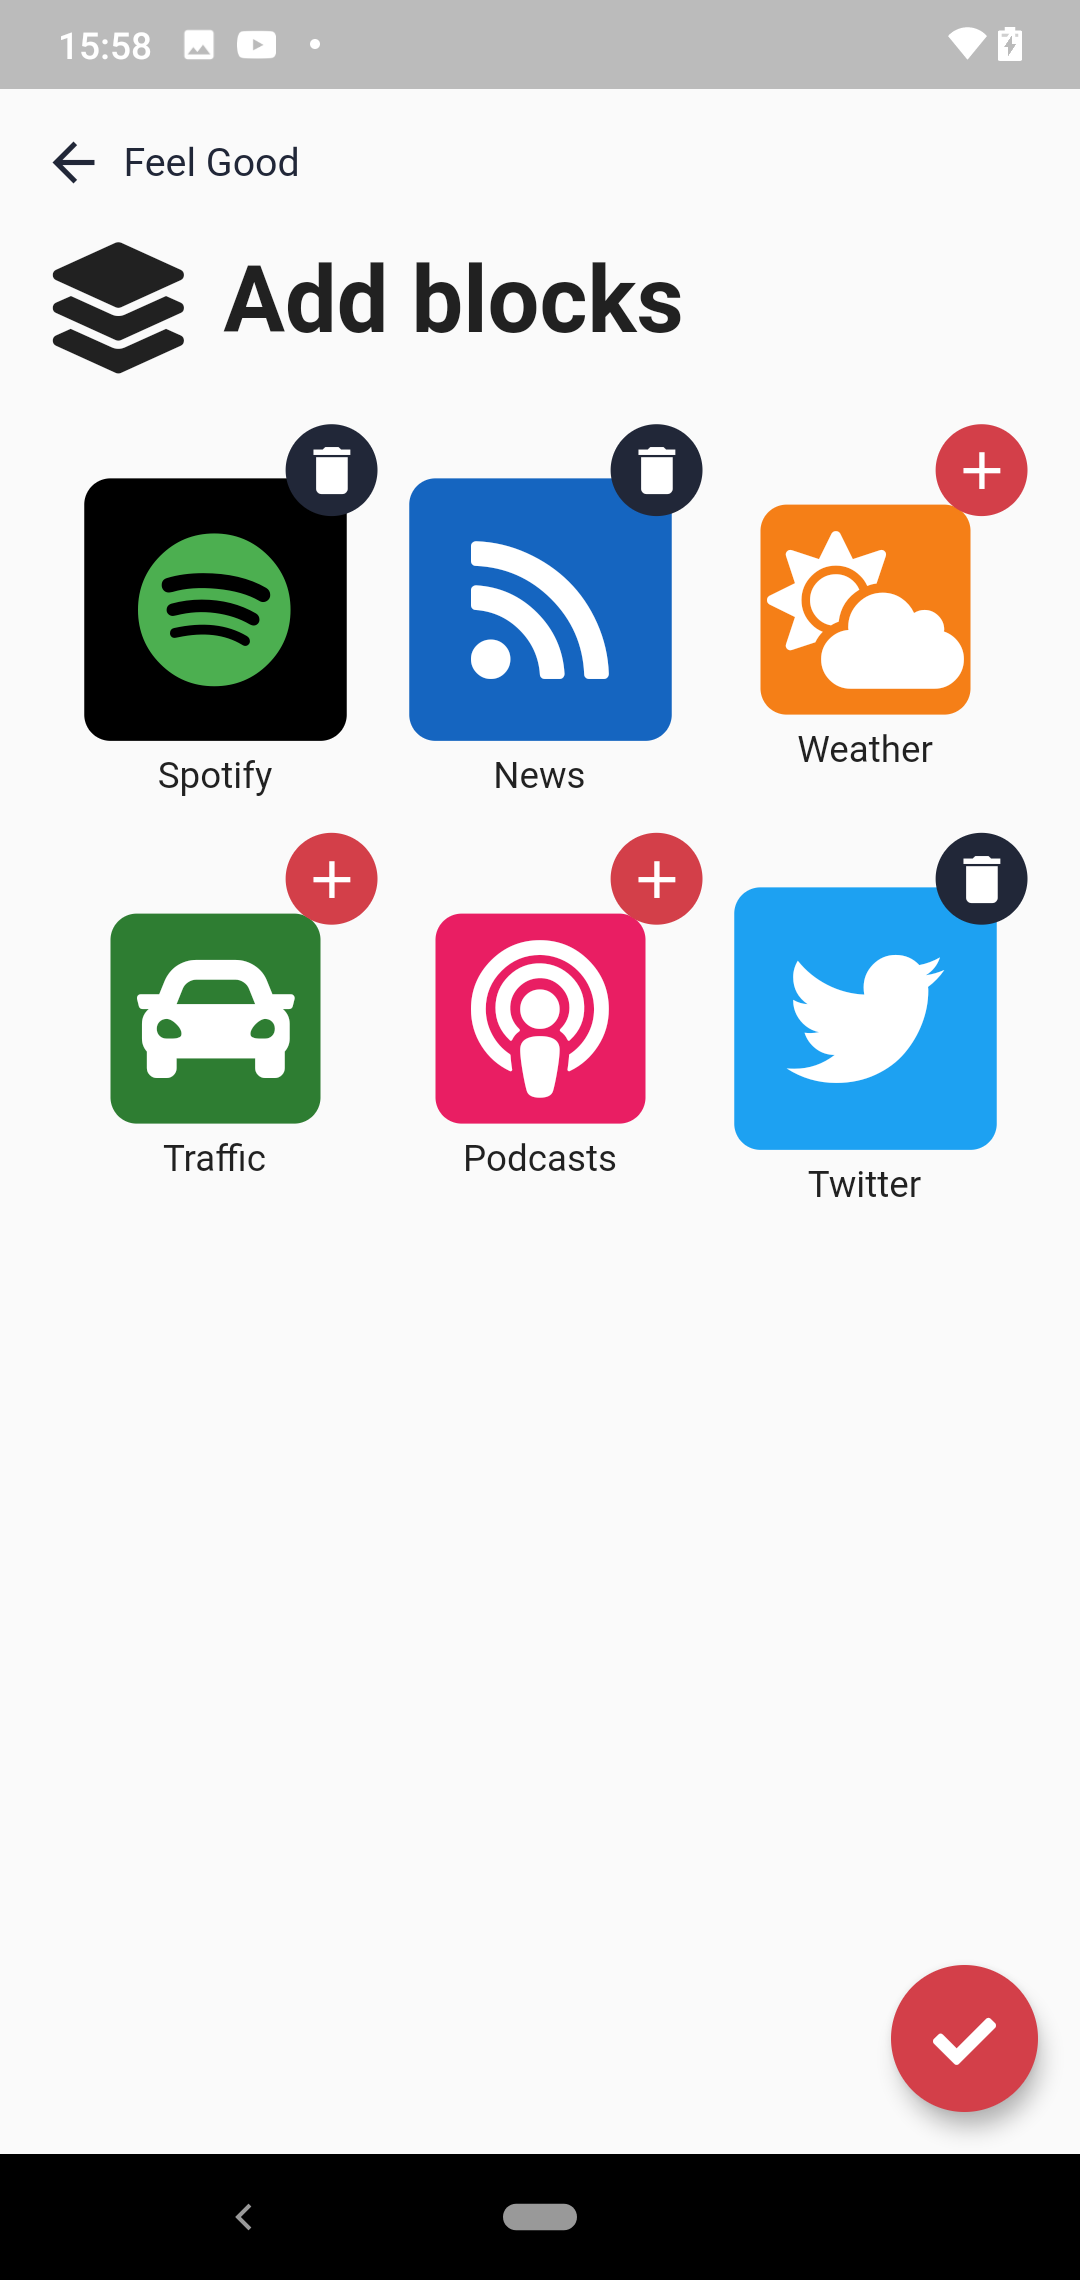
\includegraphics[width=0.29\textwidth]{./Images/screenshots/newstation2.png}}} \qquad
	\subfigure[Success screen]{\label{fig:ns3}
	\frame{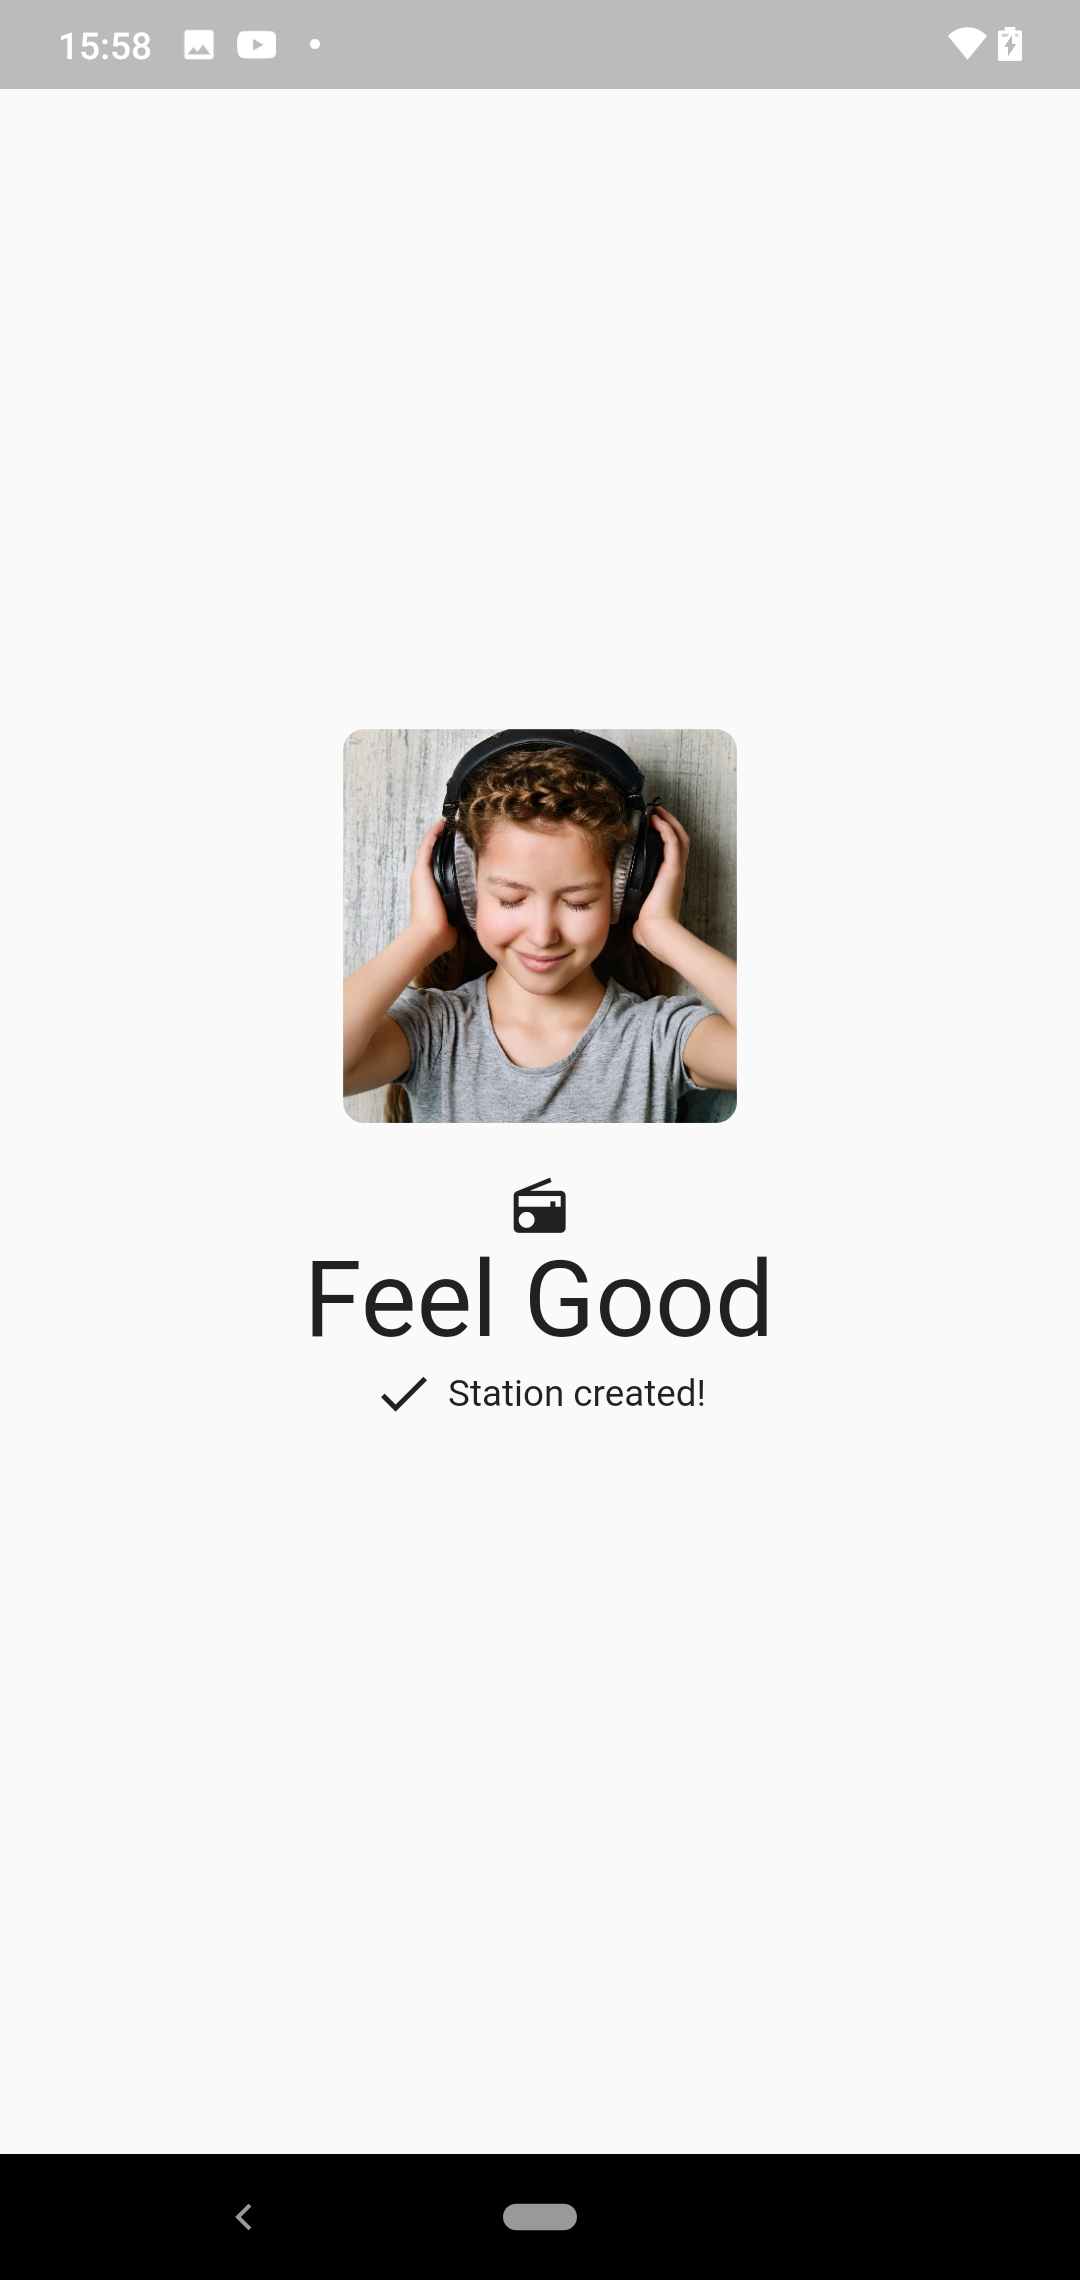
\includegraphics[width=0.29\textwidth]{./Images/screenshots/newstation3.png}}} \qquad
	\caption{Screenshots of the process of creating a new station }
	\label{fig:mfp1}
\end{figure}



\subsection{Configuring and Customizing a Station}



\begin{figure}[htbp]
	\centering
	\subfigure[Blocks screen]{\label{fig:s1}
	\frame{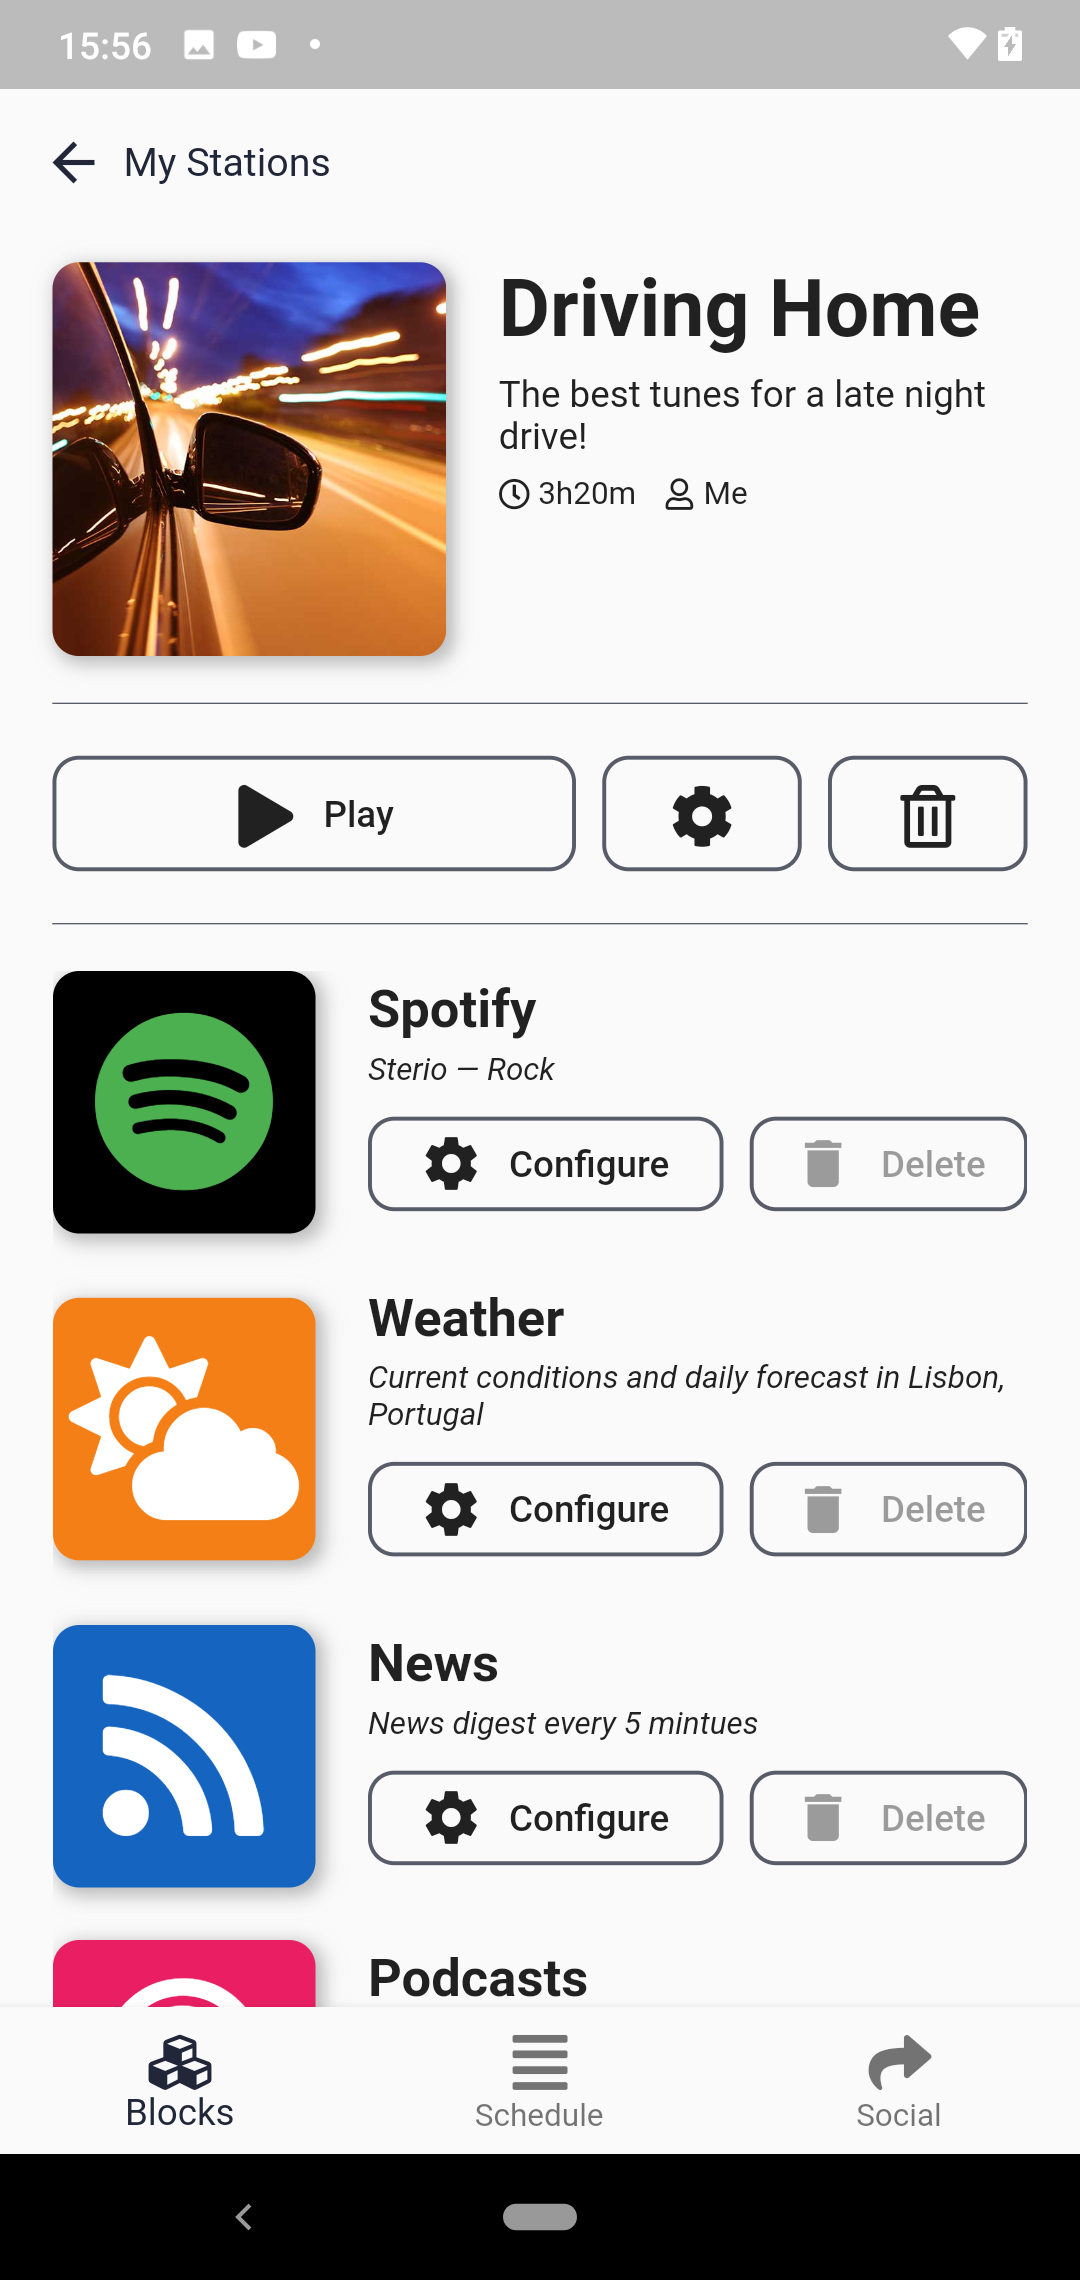
\includegraphics[width=0.29\textwidth]{./Images/screenshots/station1.png}}} \qquad
	\subfigure[Schedule screen screen]{\label{fig:s2}
	\frame{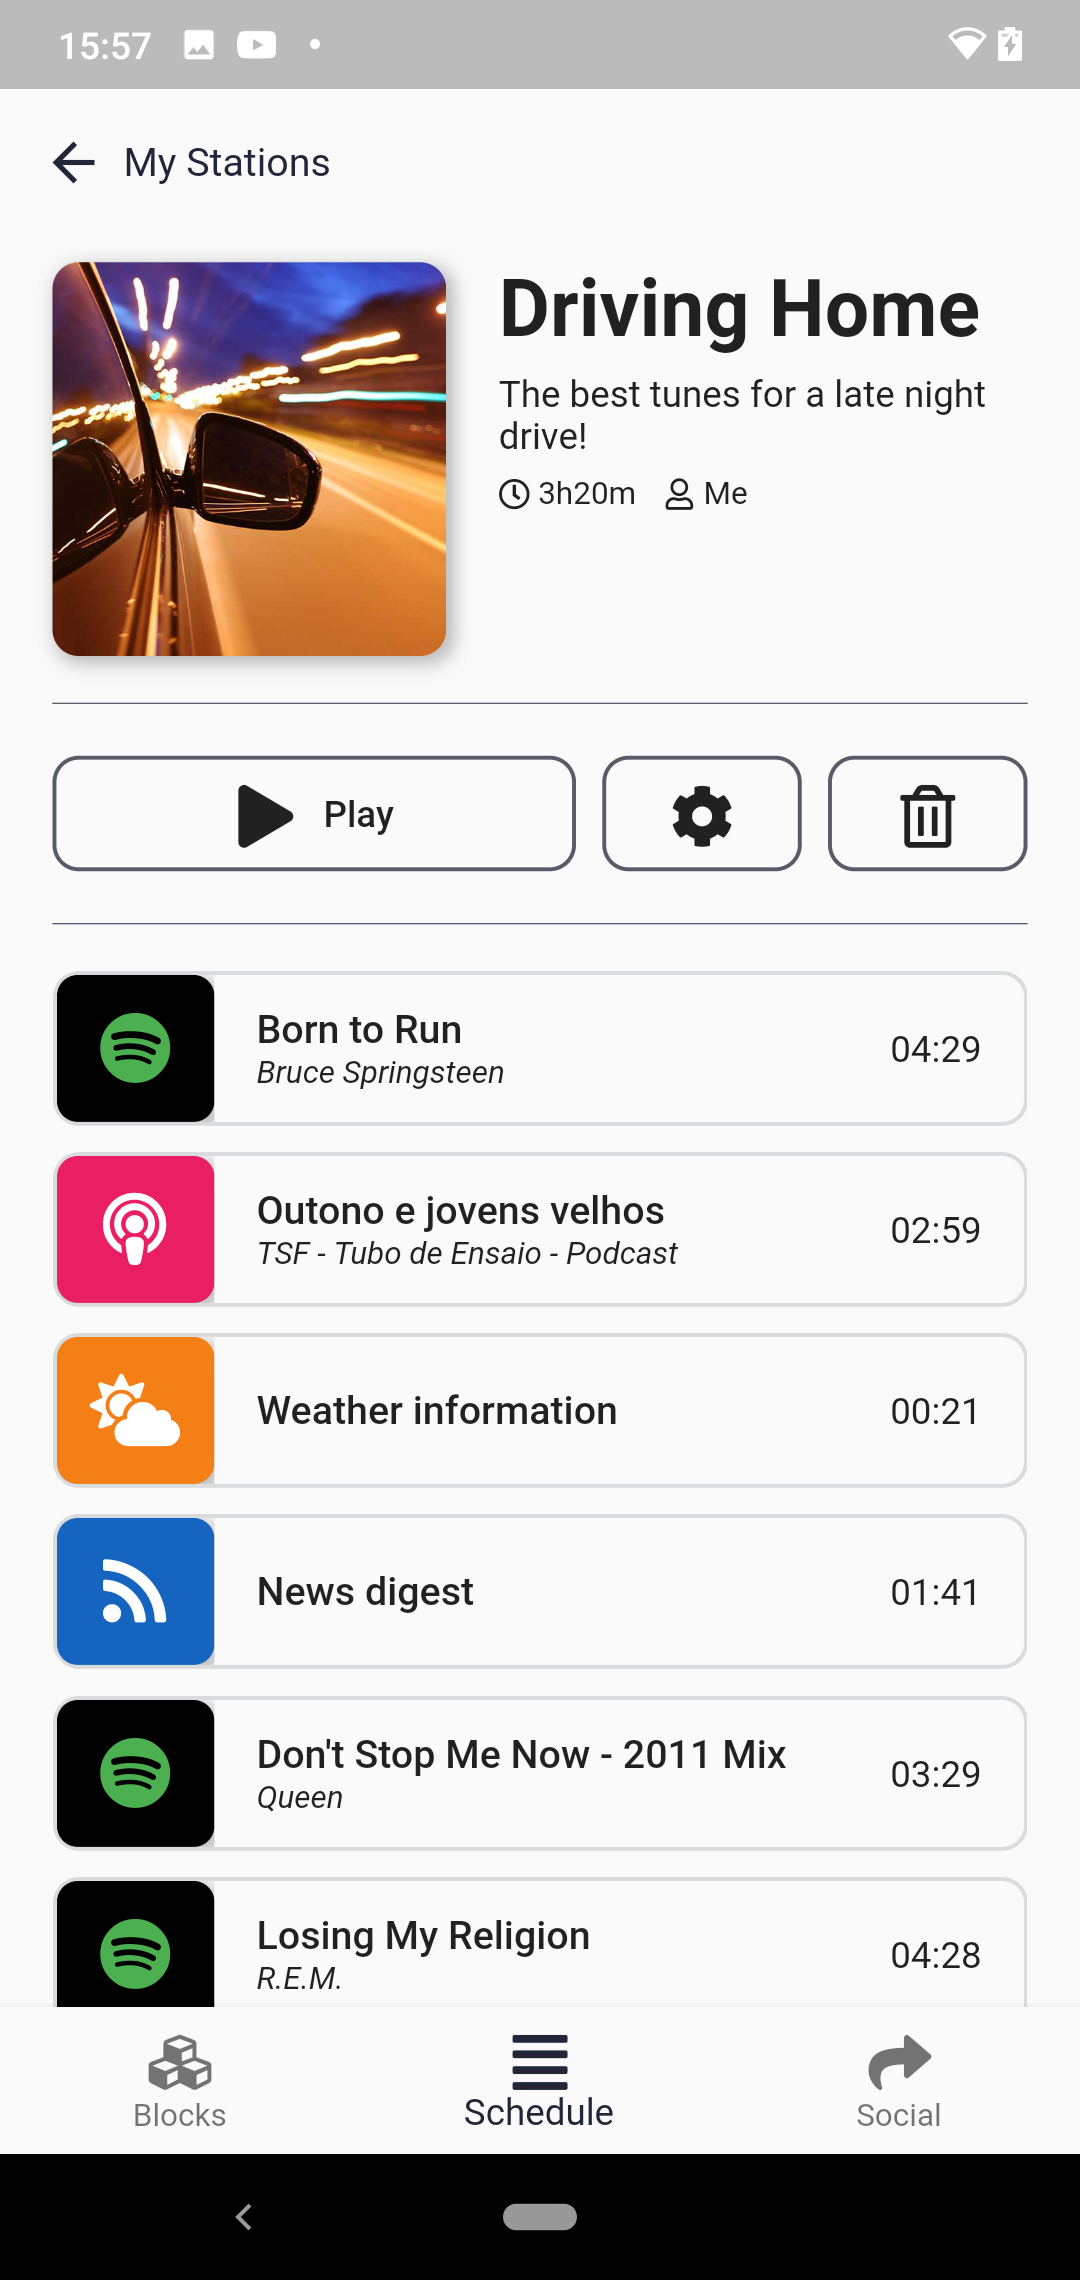
\includegraphics[width=0.29\textwidth]{./Images/screenshots/station2.png}}} \qquad
	\caption{'Driving Home' station screens}
	\label{fig:mfp1}
\end{figure}



\subsubsection{Spotify and Podcasts}

\begin{figure}[htbp]
	\centering
	\subfigure[Spotify main configuration screen]{\label{fig:spotify1}
	\frame{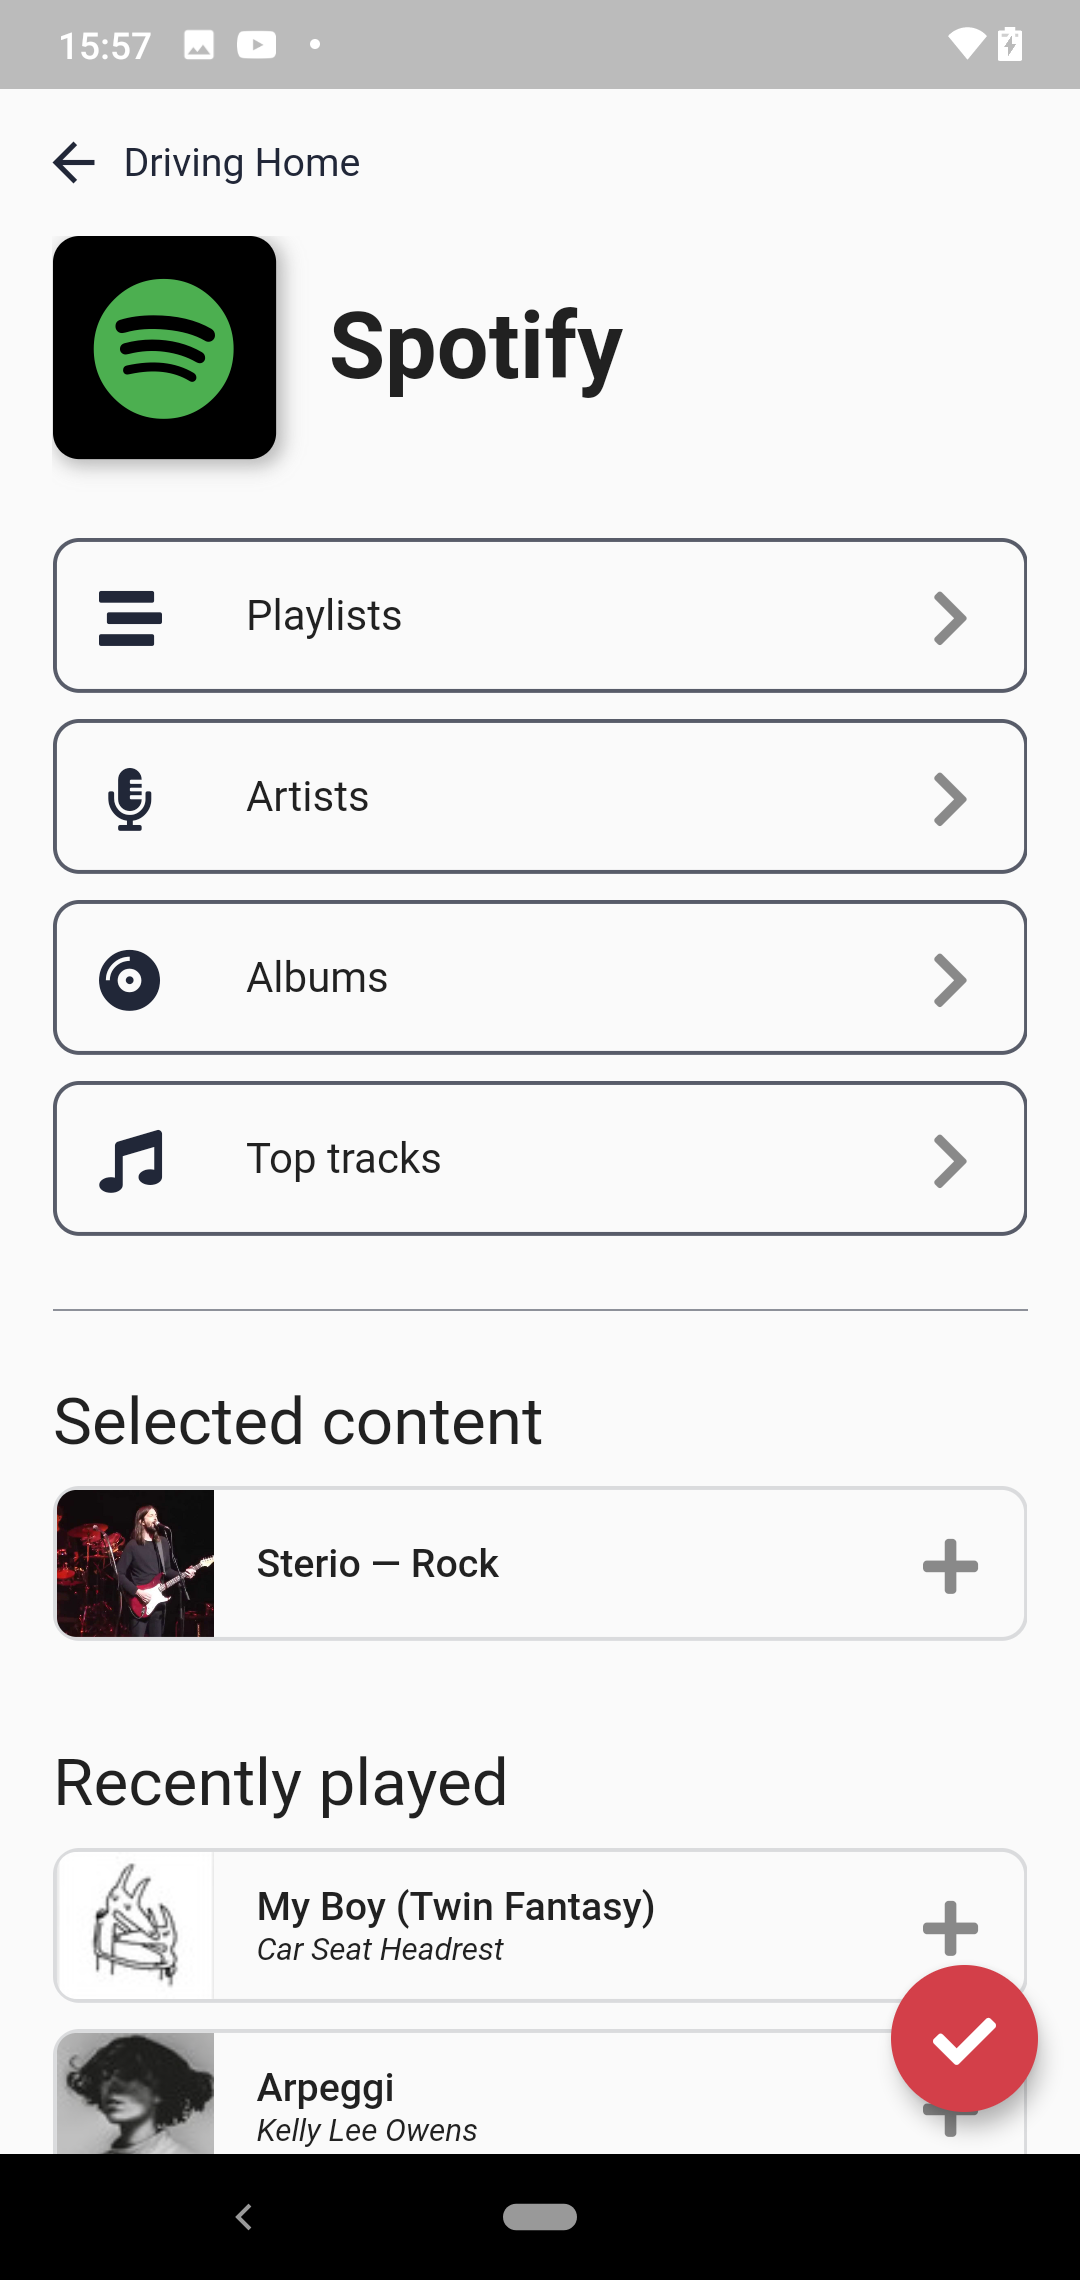
\includegraphics[width=0.29\textwidth]{./Images/screenshots/spotify.png}}} \qquad
	\subfigure[Playlists selection screen]{\label{fig:spotify2}
	\frame{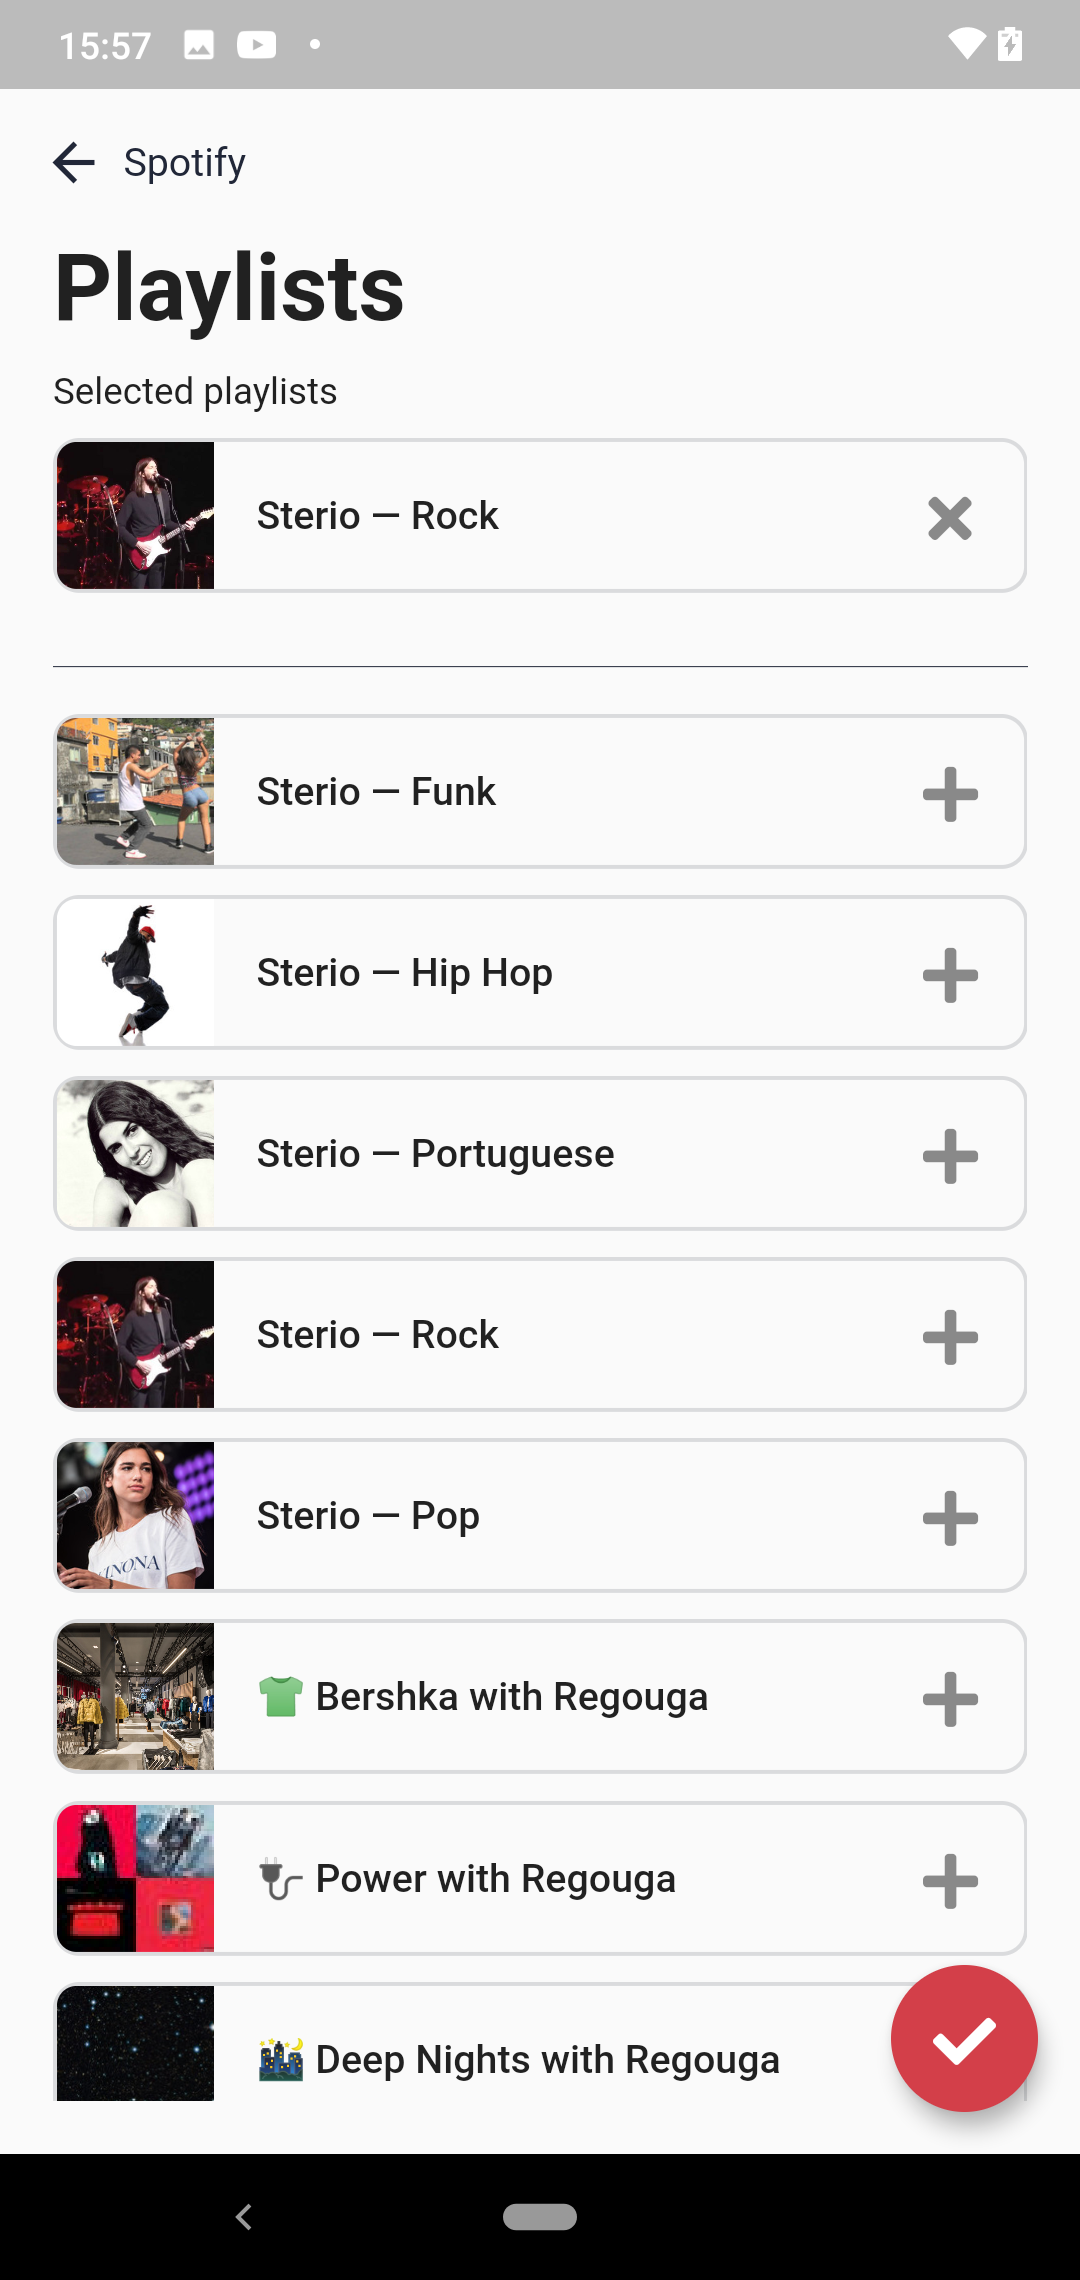
\includegraphics[width=0.29\textwidth]{./Images/screenshots/playlists.png}}} \qquad
	\caption{Spotify block configuration screens}
	\label{fig:mfp1}
\end{figure}

\subsubsection{Weather}

\begin{figure}[htbp]
	\centering
	\subfigure[Main configuration screen]{\label{fig:news1}
	\frame{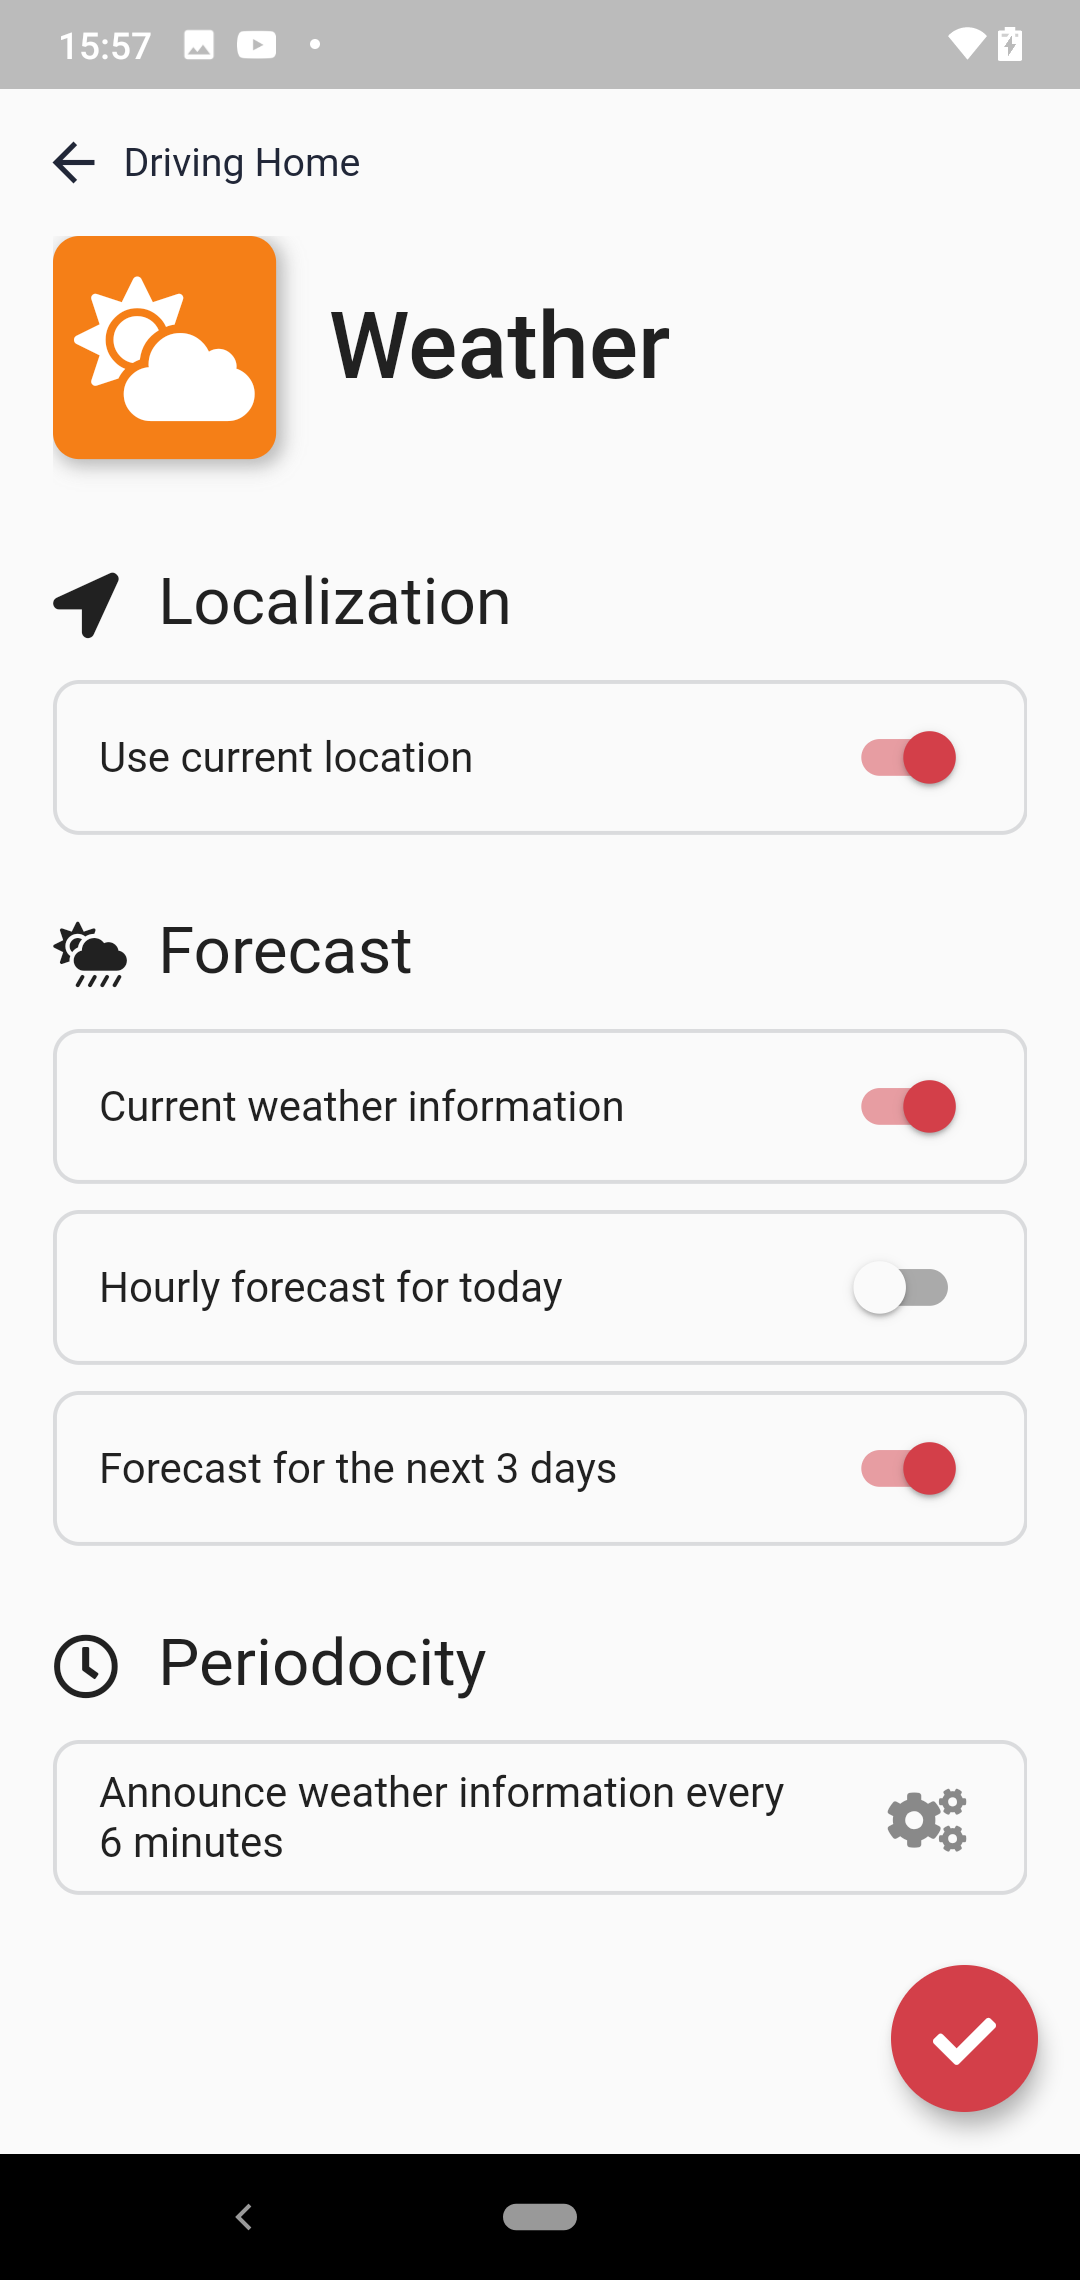
\includegraphics[width=0.29\textwidth]{./Images/screenshots/weather.png}}} \qquad
	\subfigure[Dial selector of weather periodicity]{\label{fig:news2}
	\frame{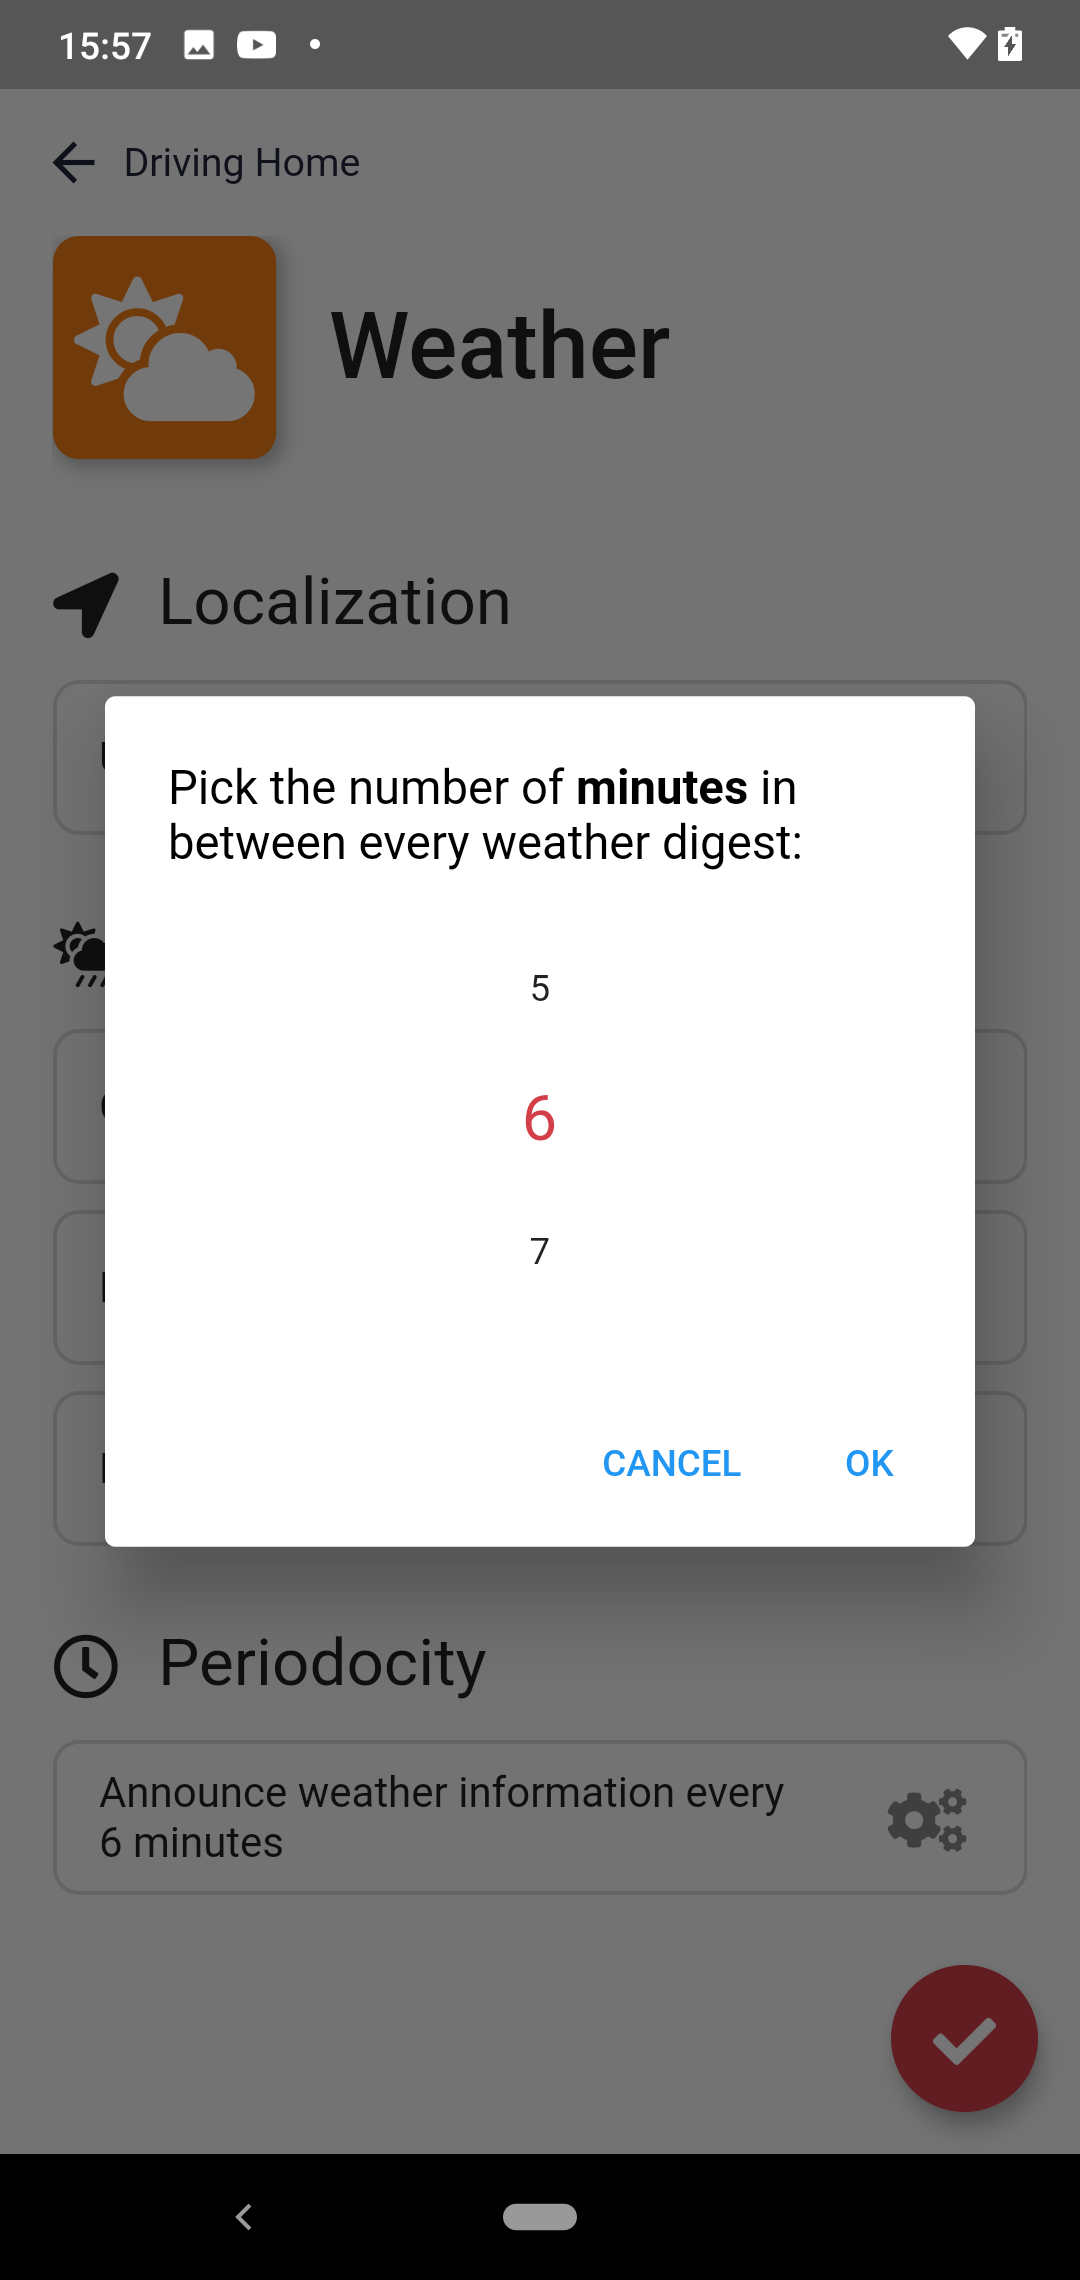
\includegraphics[width=0.29\textwidth]{./Images/screenshots/dial.png}}} \qquad
	\caption{Weather block configuration screens}
	\label{fig:weather}
\end{figure}



\subsubsection{News}

\begin{figure}[htbp]
	\centering
	\subfigure[News categories selection]{\label{fig:news1}
	\frame{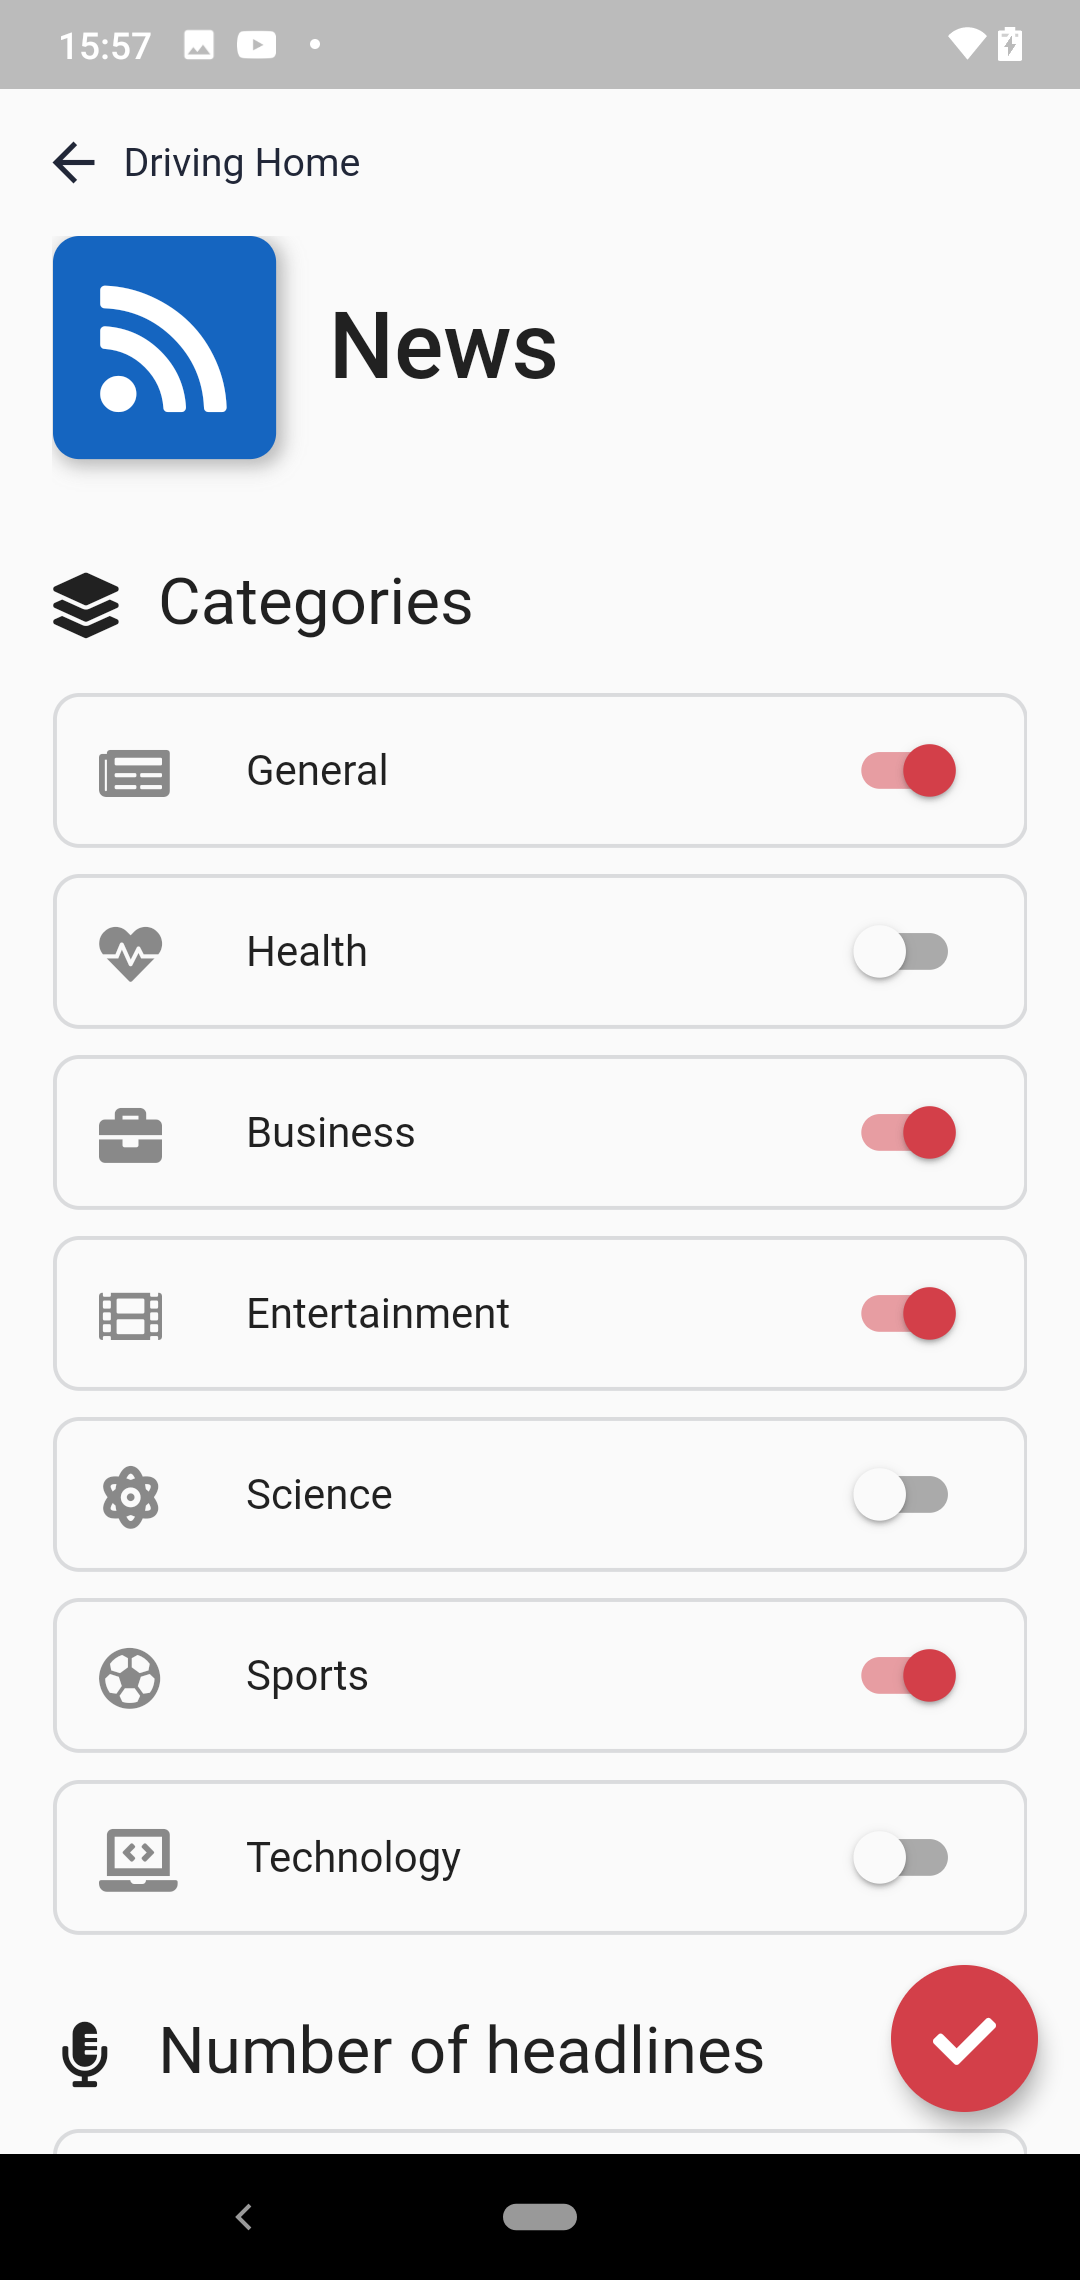
\includegraphics[width=0.29\textwidth]{./Images/screenshots/news1.png}}} \qquad
	\subfigure[Number of headlines and periodocity]{\label{fig:news2}
	\frame{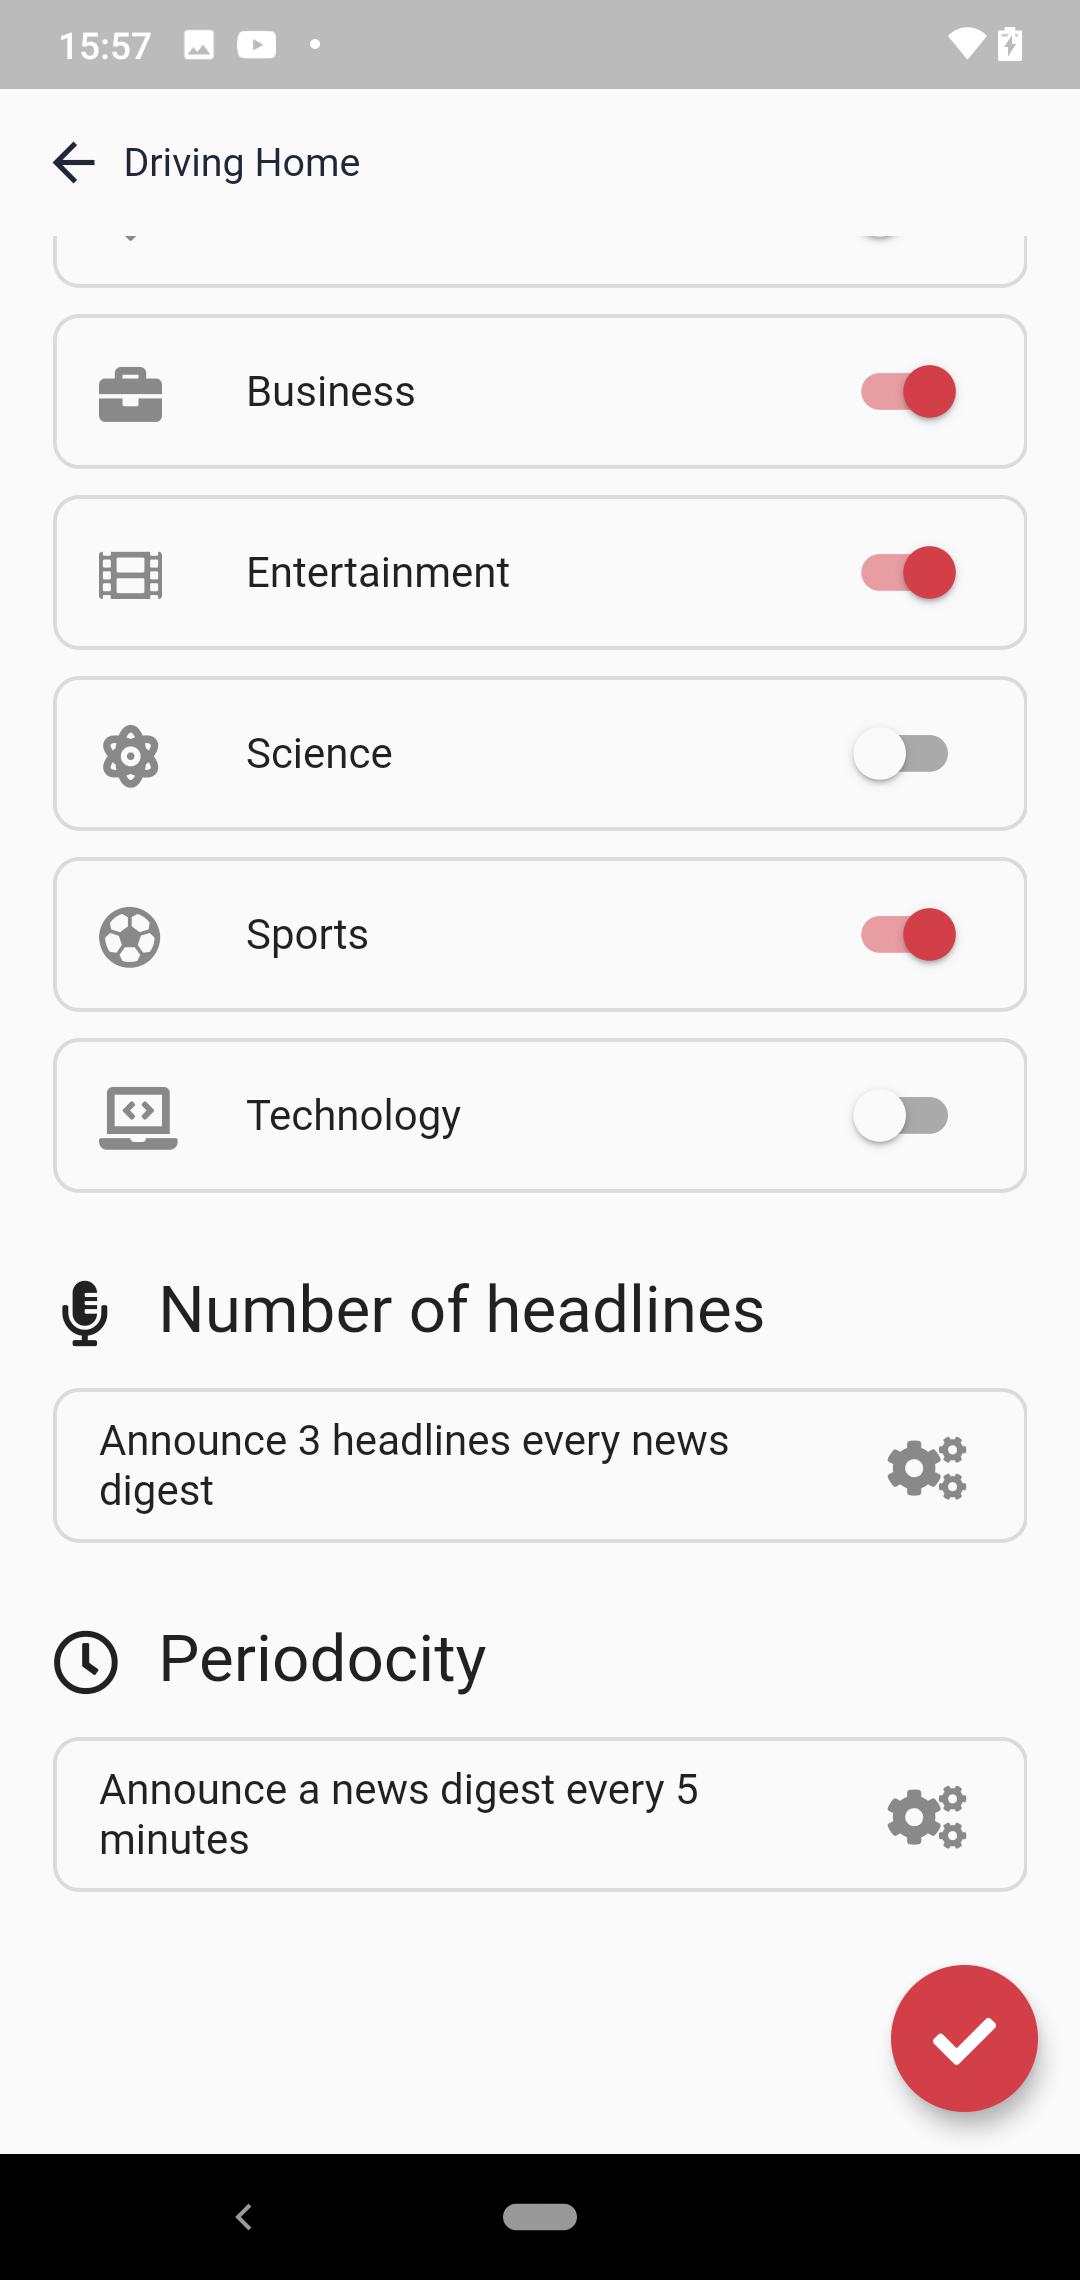
\includegraphics[width=0.29\textwidth]{./Images/screenshots/news2.png}}} \qquad
	\caption{News block configuration screens}
	\label{fig:mfp1}
\end{figure}


\subsection{Playing a Station}

\begin{figure}[htbp]
	\centering
	\subfigure[Loading ("tuning") screen]{\label{fig:play1}
	\frame{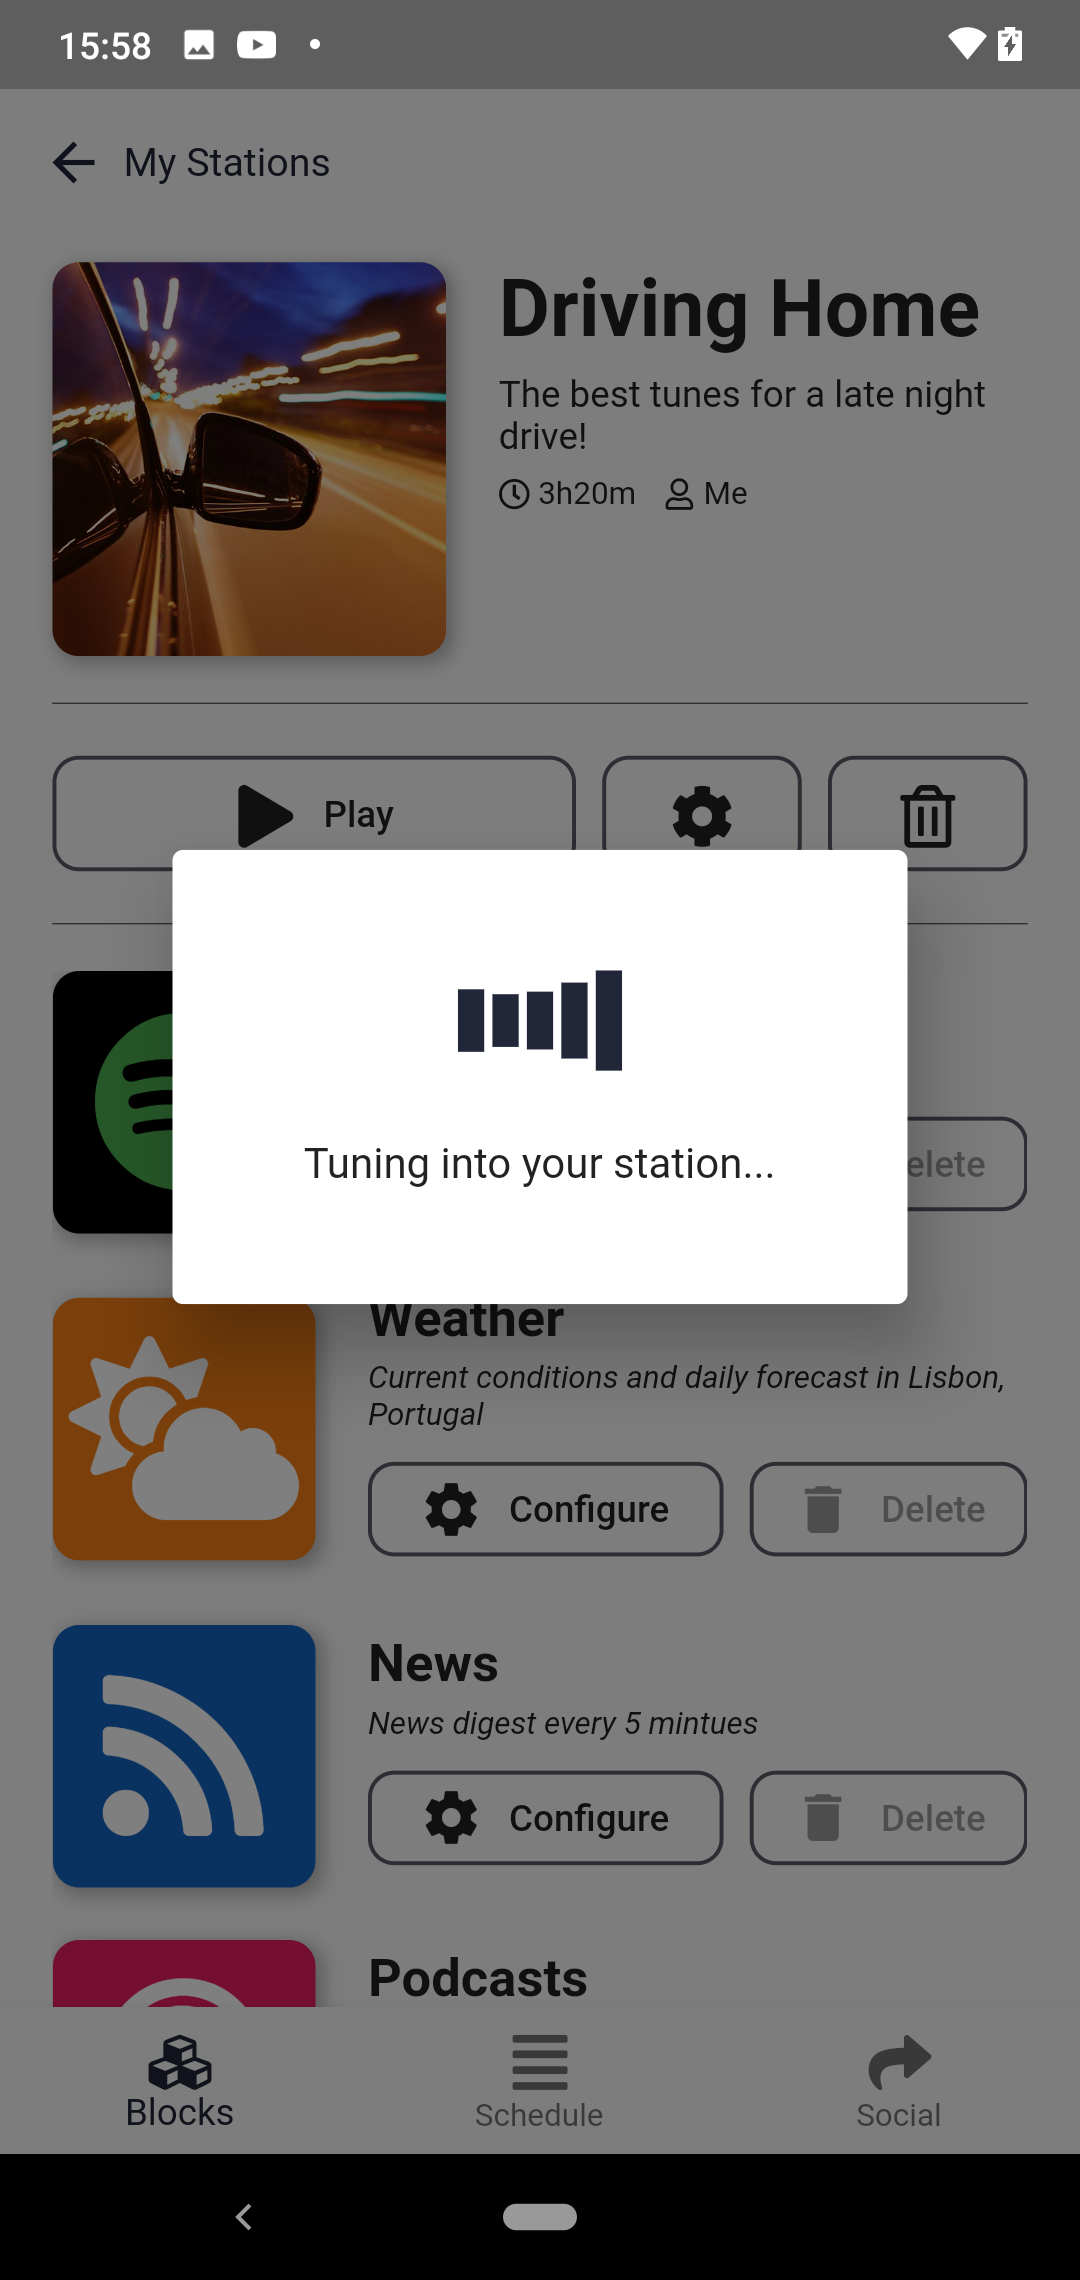
\includegraphics[width=0.29\textwidth]{./Images/screenshots/play1.png}}} \qquad
	\subfigure["Now Playing" controller bottom bar]{\label{fig:play2}
	\frame{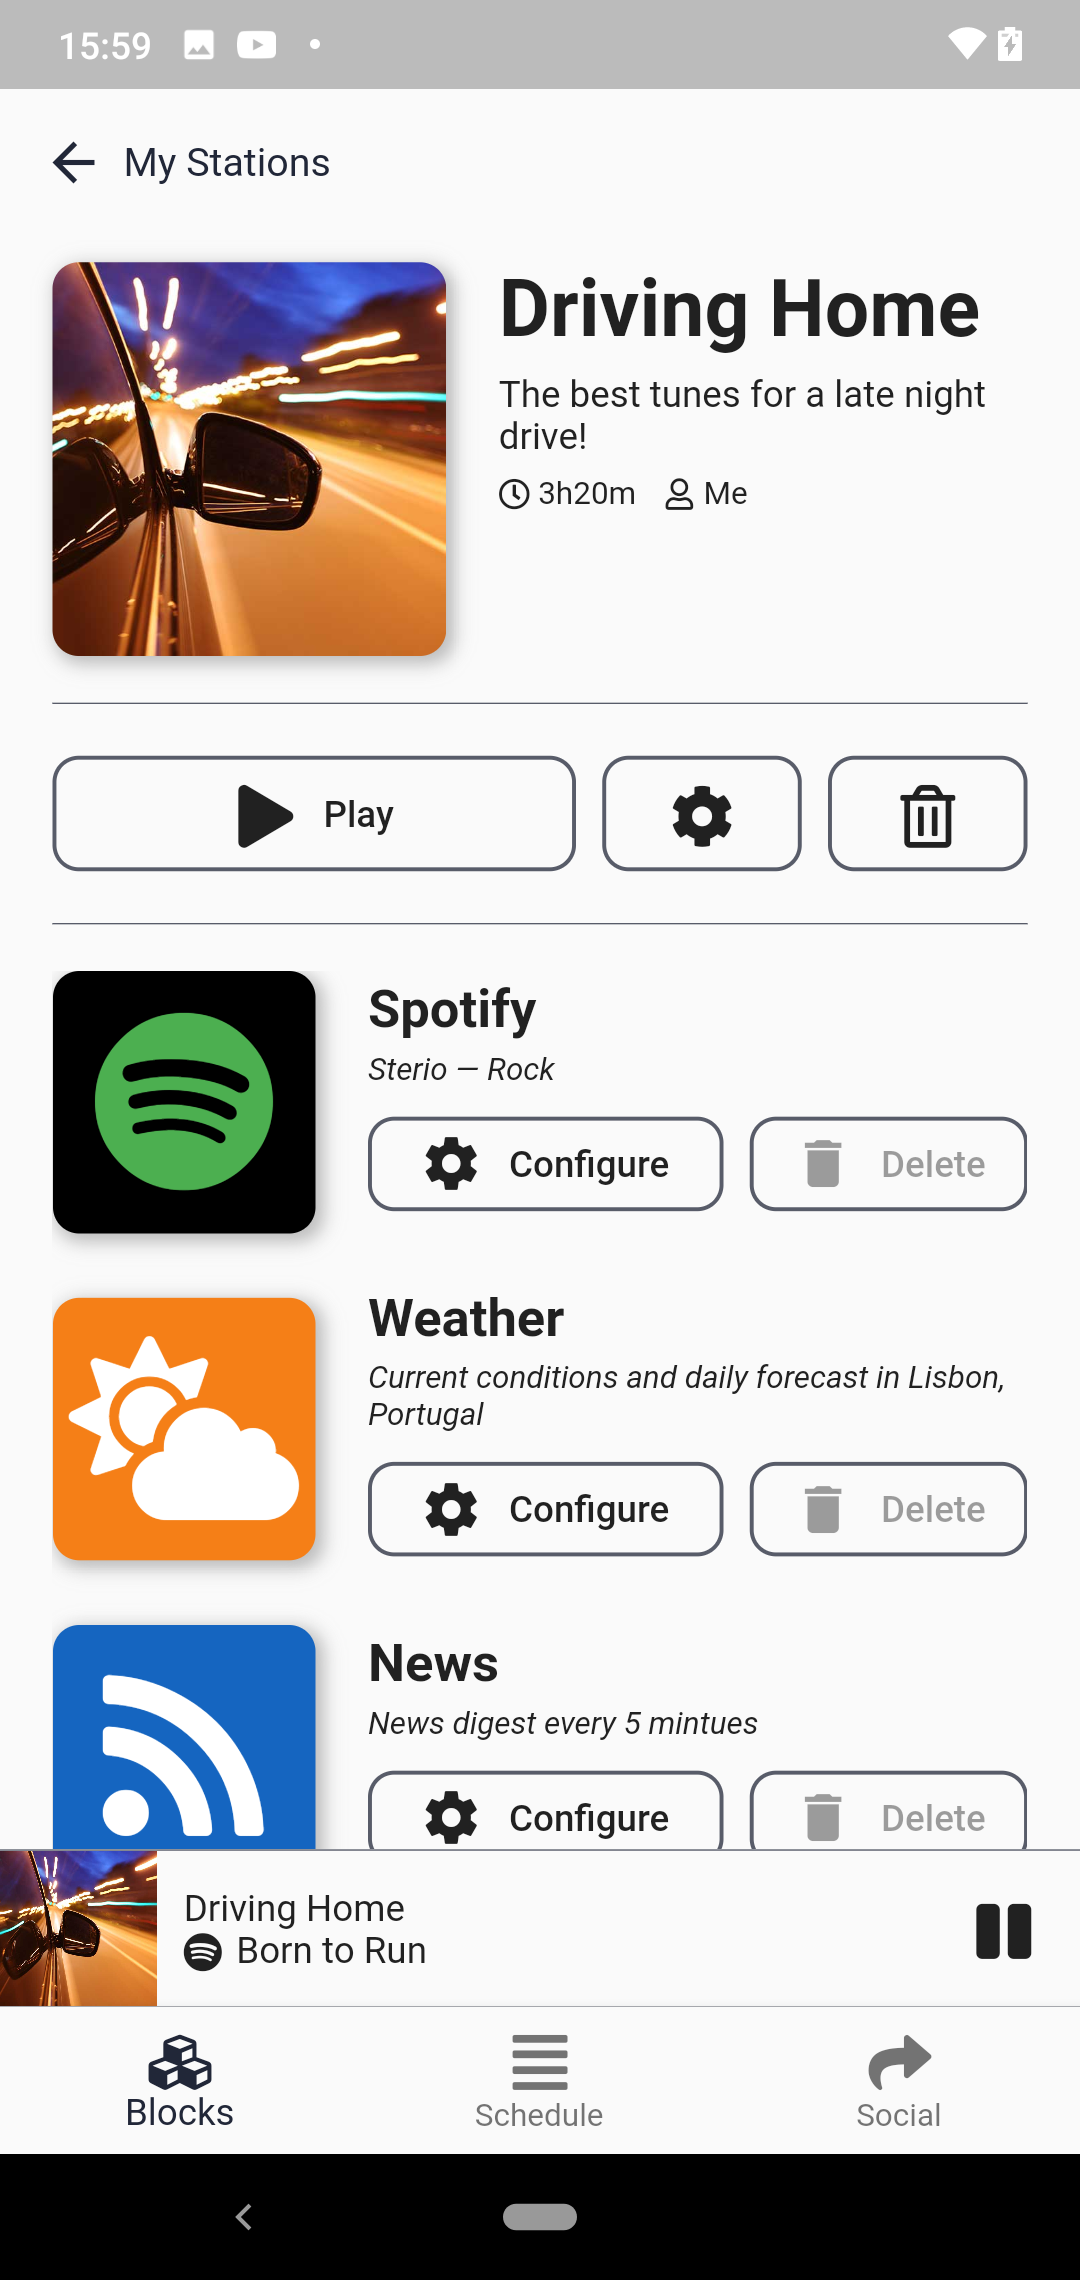
\includegraphics[width=0.29\textwidth]{./Images/screenshots/play2.png}}} \qquad
	\caption{Playing a station}
	\label{fig:mfp1}
\end{figure}

\begin{figure}[htbp]
	\centering
	\subfigure[Now playing screen]{\label{fig:np1}
	\frame{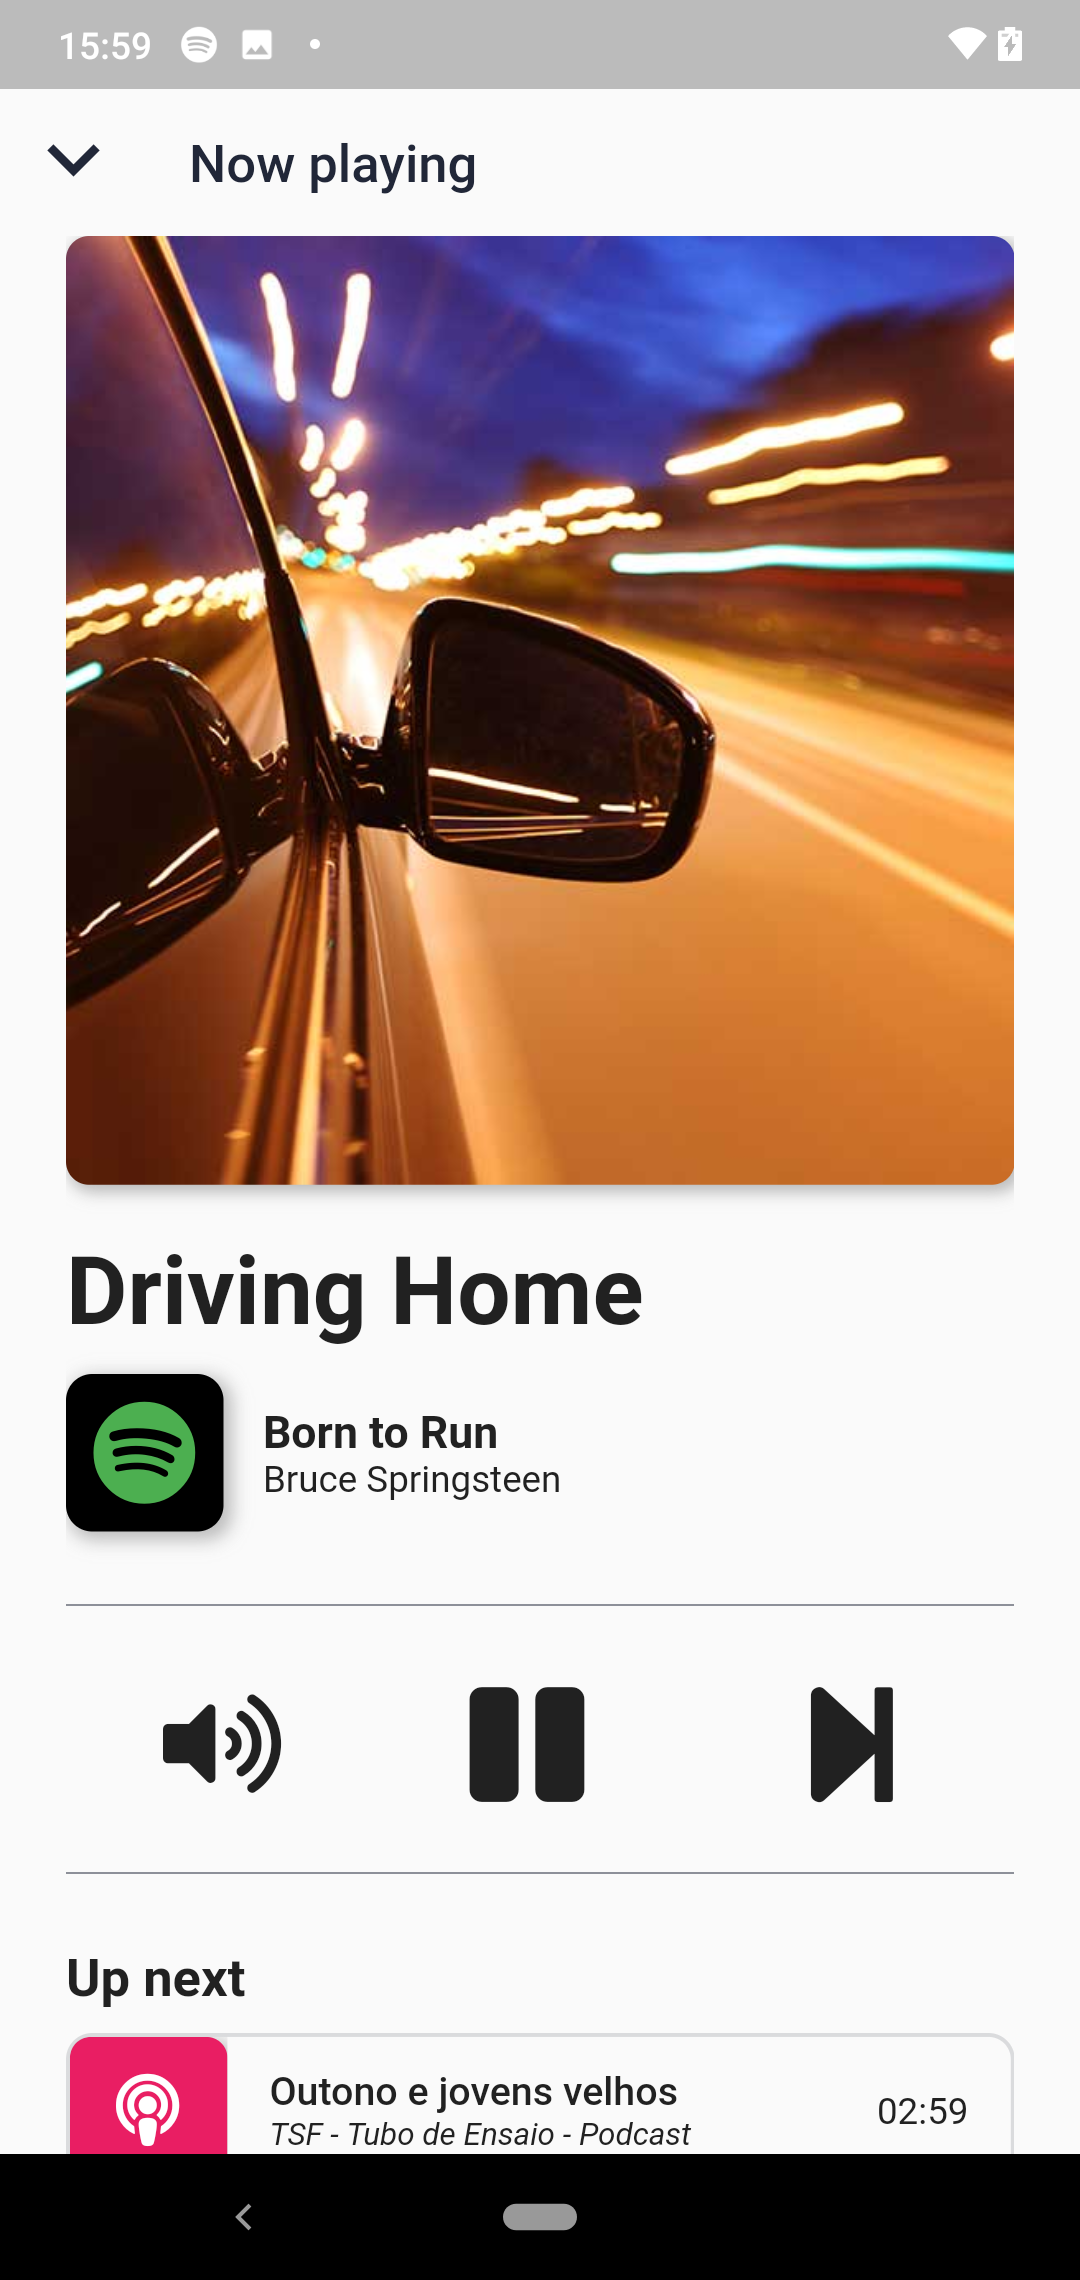
\includegraphics[width=0.29\textwidth]{./Images/screenshots/np1.png}}} \qquad
	\subfigure[Up next content]{\label{fig:np2}
	\frame{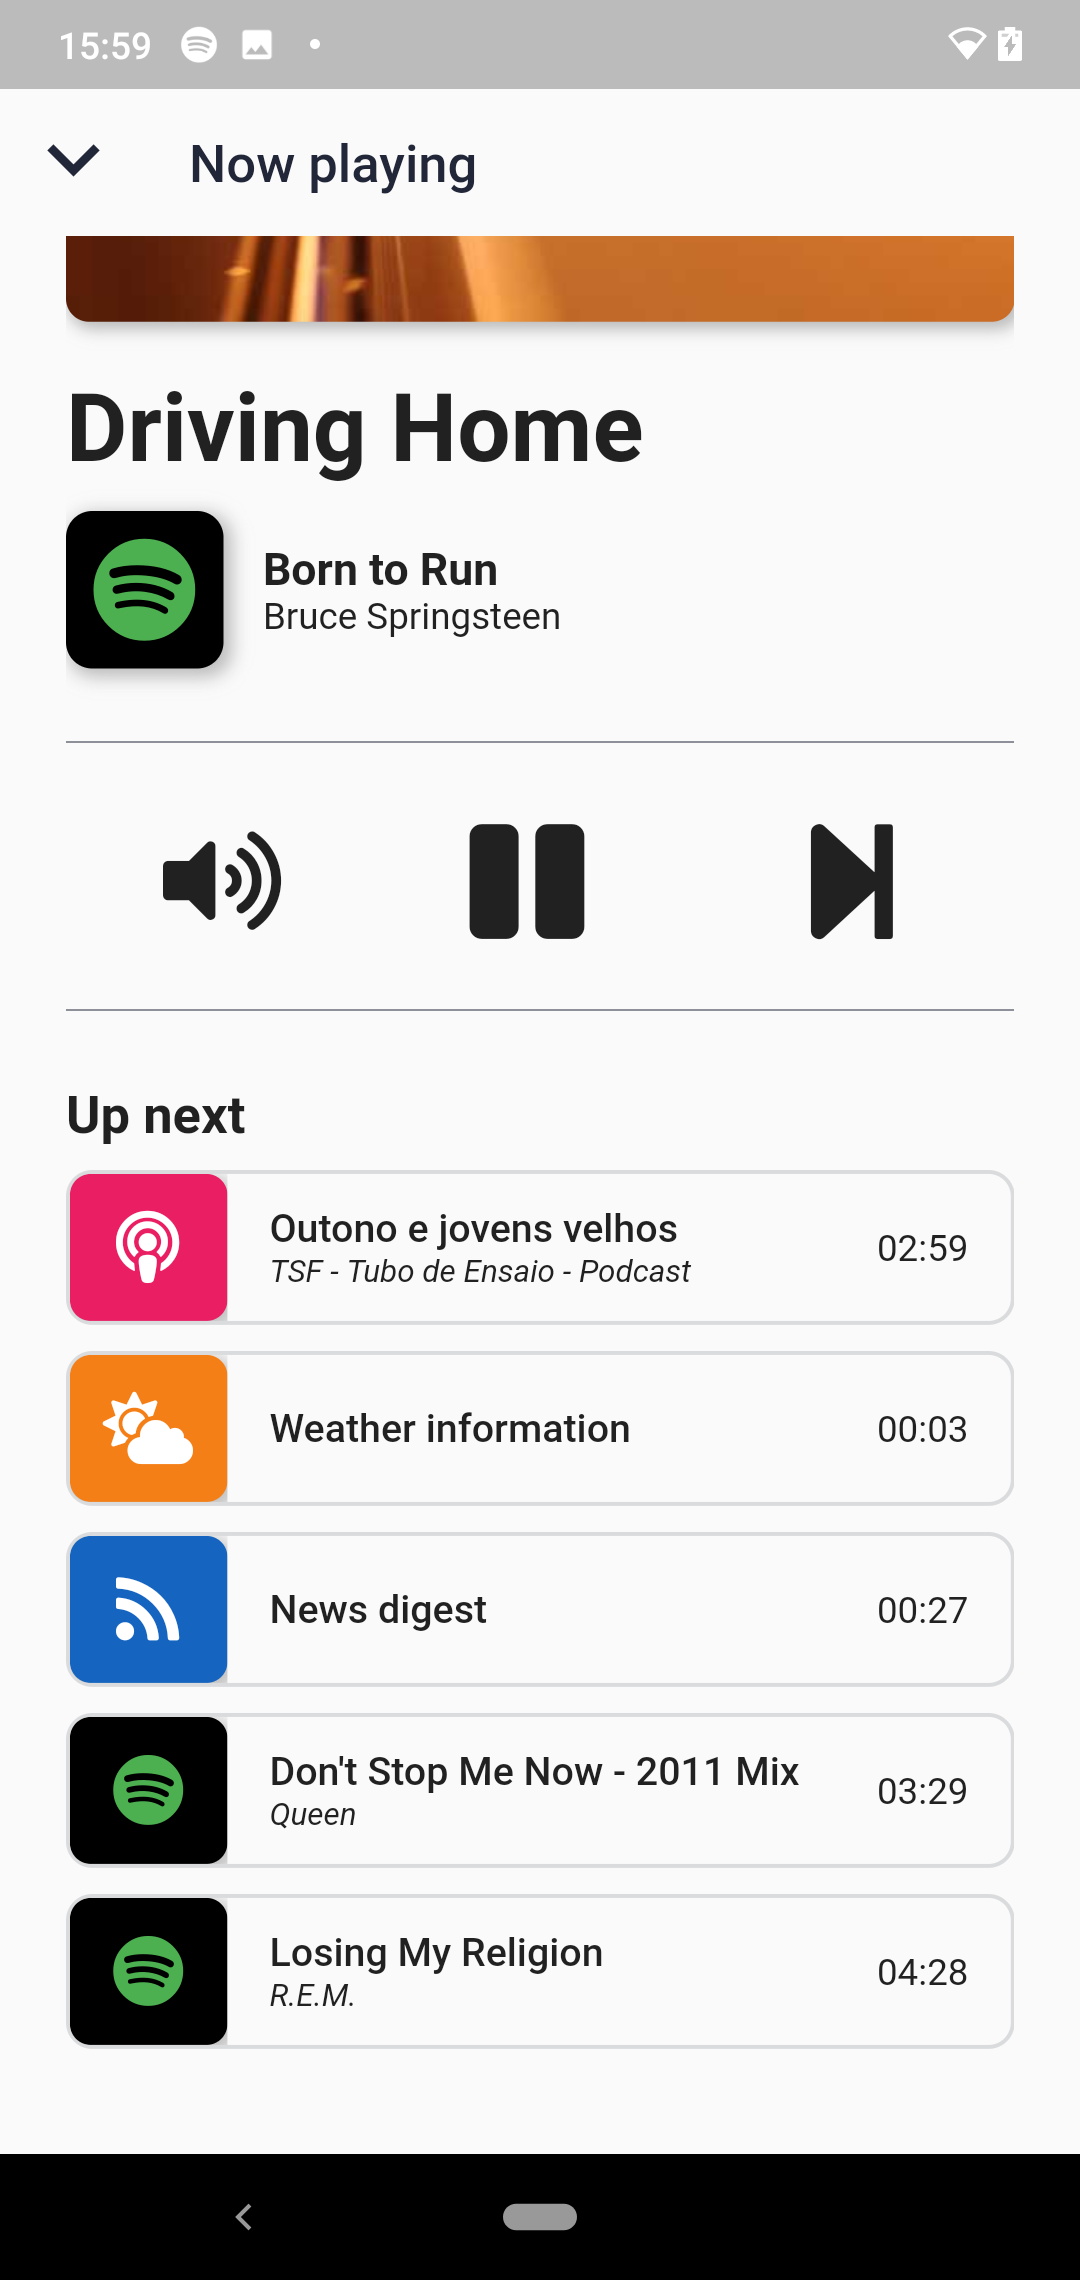
\includegraphics[width=0.29\textwidth]{./Images/screenshots/np2.png}}} \qquad
	\caption{"Now Playing" screen}
	\label{fig:mfp1}
\end{figure}


